%Copyright 2004 by Till Tantau <tantau@users.sourceforge.net>.
%
% In principle, this file can be redistributed and/or modified under
% the terms of the GNU Public License, version 2.
%
% However, this file is supposed to be a template to be modified
% for your own needs. For this reason, if you use this file as a
% template and not specifically distribute it as part of a another
% package/program, I grant the extra permission to freely copy and
% modify this file as you see fit and even to delete this copyright
% notice. 

\documentclass{beamer}
\hypersetup{pdfpagemode=FullScreen}
\usetheme{Madrid}
\usepackage[norelsize]{algorithm2e}
\usepackage{amstext} % for \text macro
\usepackage{array}   % for \newcolumntype macro
\newcolumntype{L}{>{$}l<{$}} % math-mode version of "l" column type
\usepackage{algpseudocode} % for \text macro
\usepackage{natbib}
\usepackage{svg}

%\usepackage[
%backend=biber,
%style=alphabetic,
%citestyle=authoryear 
%]{biblatex}


\usepackage{algorithm2e,float}

\usepackage{graphicx}
\usepackage{caption}
\usepackage{amsmath}
\usepackage{subfig}
\usepackage{float}
%\usepackage[round]{natbib}   % omit 'round' option if you prefer square brackets

\usepackage{empheq}
\DeclareFontFamily{OT1}{pzc}{}
\DeclareFontShape{OT1}{pzc}{m}{it}{<-> s * [1.10] pzcmi7t}{}
\DeclareMathAlphabet{\mathpzc}{OT1}{pzc}{m}{it}
\DeclareMathOperator*{\argmin}{argmin}  
\usepackage{xifthen}
\usepackage{hyperref}
\newcommand{\vect}{\bf}
\newcommand{\matr}{\bf}
%\usepackage{boadilla}
\usepackage{graphicx} % Required for including images
\graphicspath{{figs/}} % Directory in which figures are stored

\newlength\figureheight 
\newlength\figurewidth

\usepackage{float}
\usepackage{amssymb} % Adds new symbols to be used in math mode
\usepackage{wrapfig}
\usepackage{booktabs} % Top and bottom rules for tables
\usepackage{enumitem} % Used to reduce itemize/enumerate spacing
\usepackage{palatino} % Use the Palatino font
\usepackage[font=small,labelfont=bf]{caption} % Required for specifying captions to tables and figures
%\usepackage{subfig}
%\usepackage{graphicx}
\usepackage{graphicx}
\usepackage{subfig}
\usepackage{caption}
%\usepackage{tcolorbox}
\usepackage{kantlipsum}
\usepackage{etoolbox}
\AtBeginEnvironment{algorithm}{%
	\setlength{\columnwidth}{\linewidth}%
}
\pgfmathdeclarefunction{gauss}{2}{%
	\pgfmathparse{1/(#2*sqrt(2*pi))*exp(-((x-#1)^2)/(2*#2^2))}%
}

%\usepackage[usenames, dvipsnames]{color}
%\newlength\mytemplen
%\newsavebox\mytempbox
%\definecolor{myblue}{rgb}{.8, .8, 1}
%\newcommand\mybluebox{%
%	\@ifnextchar[%]
%	{\@mybluebox}%
%	{\@mybluebox[0pt]}}
%
%\def\@mybluebox[#1]{%
%	\@ifnextchar[%]
%	{\@@mybluebox[#1]}%
%	{\@@mybluebox[#1][0pt]}}
%
%\def\@@mybluebox[#1][#2]#3{
%	\sbox\mytempbox{#3}%
%	\mytemplen\ht\mytempbox
%	\advance\mytemplen #1\relax
%	\ht\mytempbox\mytemplen
%	\mytemplen\dp\mytempbox
%	\advance\mytemplen #2\relax
%	\dp\mytempbox\mytemplen
%	\colorbox{myblue}{\hspace{1em}\usebox{\mytempbox}\hspace{1em}}}


%\definecolor{lightblue}{rgb}{0.145,0.6666,1} % Defines the color used for content box headers
%\newcommand\Fontvi{\fontsize{6}{7.2}\selectfont}
\newcommand\Fontvi[3][2]{\fontsize{#2pt}{#3pt}\selectfont}


\newcommand{\compresslist}{ % Define a command to reduce spacing within itemize/enumerate environments, this is used right after \begin{itemize} or \begin{enumerate}
\setlength{\itemsep}{1pt}
\setlength{\parskip}{0pt}
\setlength{\parsep}{0pt}
}
\renewcommand{\footnotesize}{\fontsize{7.5pt}{9pt}\selectfont}
%\usepackage{enumitem}
\newcommand{\sxx}[1]{{\color{red} - S: #1 - \ }}  % Suman's comments
\newcommand{\axx}[1]{{\color{orange} - #1 - \ }}
\newcommand{\tl}[1]{{\color{orange} - Fix Language: #1 - \ }}  % Typo or Language
\newcommand{\bxx}[1]{{\color{blue} - T: #1 - \ }}  % AmirHossein's comments
\newcommand{\bc}[1]{{\color{blue}  #1  }}  % AmirHossein's comments
\newcommand{\rc}[1]{{\color{red}  #1  }}  % AmirHossein's comments
\newcommand{\gc}[1]{{\color{green}  #1  }}  % AmirHossein's comments
\newcommand{\bIs}[1]{\boldsymbol{I}_{#1}}  % Suman's comments


\theoremstyle{remark}
\newtheorem{remark}{Remark}
% and optionally (as of Pgfplots 1.3): 
\usepackage{pgfplots} 

\pgfplotsset{compat=newest} 
\pgfplotsset{plot coordinates/math parser=false} 
%\renewcommand{\footnotesize}{\footnotesize}
\renewcommand{\footnotesize}{\fontsize{7.5pt}{9pt}\selectfont}
%\usepackage{enumitem}

\newcommand{\XX}[3][2]{\mathbf{X}_{\tiny #2}^{\tiny #3}}
\newcommand{\pr}{\textrm{p}}
\newcommand{\pp}[3][2]{\pr(x #2 | #3)}



\newcommand{\bIn}{\boldsymbol{I}_{\boldsymbol{n}}}
\newcommand{\bIa}{\boldsymbol{I}_{\boldsymbol{a}}}
\newcommand{\bIk}{\boldsymbol{I}_{\boldsymbol{k}}}
\newcommand{\bIkk}{\boldsymbol{I}_{\boldsymbol{k-1}}}

\newcommand{\xx}[3][2]{\mathbf{x}_{ #2}^{ #3}}
\newcommand{\zz}[3][2]{\mathbf{z}_{ #2}^{ #3}}
\newcommand{\ZZ}[3][2]{\mathbf{Z}_{ #2}^{ #3}}
\newcommand{\ZZh}[3][2]{\mathbf{\hat{z}}_{ #2}^{ #3}}
%\newcommand{\yy}[3][2]{\mathpzc{y}_{\tiny #2}^{\tiny #3}}
%\newcommand{\YY}[3][2]{\mathpzc{Y}_{\tiny #2}^{\tiny #3}}

\newcommand{\yy}[3][2]{\psi^{\tiny #3}({\tiny #2})}
\newcommand{\YY}[3][2]{\phi^{\tiny #3}({\tiny #2})}
\newcommand{\suf}[1]{\textsc{\tiny #1}}  % Suman's comments

\newcommand{\ii}[3][2]{\overline{\delta \mathpzc{i}}_{\tiny {#2}}^{\tiny {#3}}}
\newcommand{\II}[3][2]{\overline{\delta \mathpzc{I}}_{\tiny {#2}}^{\tiny {#3}}}
\newcommand{\psx}{p_*(\vect{x})}
\newcommand{\pcfx}{p_{\textsc{\tiny CF}}(\vect{x})}
\newcommand{\phybx}{p_{\textsc{\tiny HYB}}(\vect{x})}
\newcommand{\pixz}{\tilde{p}^i(\xx[]{k}{}\vert \vect{Z}_{k})}
\newcommand{\pixzm}{\tilde{p}^i(\xx[]{k}{}\vert \vect{Z}_{k-1})}
\newcommand{\pzix}{\tilde{p}^i( \vect{z}_{k} \vert \xx[]{k}{})}
\newcommand{ \pcf}{\frac{1}{\eta_{\textsuperscript{CF}}}\prod_{i=1}^{N} \pr(\vect{z}_{k}^i | \xx[]{k}{})^{\omega_i} \prod_{i=1}^{N} \tilde{p}^i(\vect{x}_{k} | \vect{Z}_{k-1})^{\omega_i}}
\newcommand{ \phyb}{\frac{1}{\eta_{\textsc{\tiny HYB}}}\prod_{i=1}^{N} \pr(\vect{z}_{k}^i | \xx[]{k}{}) \prod_{i=1}^{N} \tilde{p}^i(\vect{x}_{k} | \vect{Z}_{k-1})^{\bar{\omega}_i} }
\newcommand{ \pstar}{\frac{1}{\eta_*} \{ \prod_{i=1}^{N} \pr(\vect{z}_{k}^i | \xx[]{k}{}) \} \pr(\xx[]{k}{}|\vect{Z}_{k-1})}

\newcommand{ \npcf}{\prod_{i=1}^{N} \pr(\vect{z}_{k}^i | \xx[]{k}{})^{\omega_i} \prod_{i=1}^{N} \tilde{p}^i(\vect{x}_{k} | \vect{Z}_{k-1})^{\omega_i}}
\newcommand{ \nphyb}{\prod_{i=1}^{N} \pr(\vect{z}_{k}^i | \xx[]{k}{}) \prod_{i=1}^{N} \tilde{p}^i(\vect{x}_{k} | \vect{Z}_{k-1})^{\bar{\omega}_i} }
\newcommand{ \npstar}{ \{ \prod_{i=1}^{N} \pr(\vect{z}_{k}^i | \xx[]{k}{}) \} \pr(\xx[]{k}{}|\vect{Z}_{k-1})}


\DeclareDocumentCommand{\ais}{m m m  }{{#1}_{#2}^{#3}}
\DeclareDocumentCommand{\bis}{m m m  }{{#1}_{{\tiny #2}}^{{\tiny #3}}}
\DeclareDocumentCommand{\cis}{m m m  }{{#1}_{{\tiny #2}}^{{\tiny {#3}}}}
\newcommand{\ti}[1]{\textsc{\tiny #1}}
\newcommand{\lrp}[1]{\left( #1 \right) }



\DeclareDocumentCommand{\ais}{m m m  }{{#1}_{#2}^{#3}}
\DeclareDocumentCommand{\bis}{m m m  }{{#1}_{{\tiny #2}}^{{\tiny #3}}}
\DeclareDocumentCommand{\cis}{m m m  }{{#1}_{{\tiny #2}}^{{\ti{#3}}}}







%\newcommand{\yy}[3][2]{\mathpzc{y}_{\tiny #2}^{\tiny #3}}
%\newcommand{\YY}[3][2]{\mathpzc{Y}_{\tiny #2}^{\tiny #3}}



\usepackage{multicol} % Required for multiple columns
\setlength{\columnsep}{1.5em} % Slightly increase the space between columns
\setlength{\columnseprule}{0mm} % No horizontal rule between columns

\usepackage{tikz} % Required for flow chart
\usetikzlibrary{shapes,arrows} % Tikz libraries required for the flow chart in the template

\usepackage{algpseudocode}% http://ctan.org/pkg/algorithmicx
\usepackage{microtype}

% There are many different themes available for Beamer. A comprehensive
% list with examples is given here:
% http://deic.uab.es/~iblanes/beamer_gallery/index_by_theme.html
% You can uncomment the themes below if you would like to use a different
% one:
%\usetheme{AnnArbor}
%\usetheme{Antibes}
%\usetheme{Bergen}
%\usetheme{Berkeley}
%\usetheme{Berlin}
%\usetheme{Boadilla}
%\usetheme{boxes}
%\usetheme{CambridgeUS}
%\usetheme{Copenhagen}
%\usetheme{Darmstadt}
%\usetheme{default}
%\usetheme{Frankfurt}
%\usetheme{Goettingen}
%\usetheme{Hannover}
%\usetheme{Ilmenau}
%\usetheme{JuanLesPins}
%\usetheme{Luebeck}
\usetheme{Madrid}
%\usetheme{Malmoe}
%\usetheme{Marburg}
%\usetheme{Montpellier}
%\usetheme{PaloAlto}
%\usetheme{Pittsburgh}
%\usetheme{Rochester}
%\usetheme{Singapore}
%\usetheme{Szeged}
%\usetheme{Warsaw}

\title{Efficient Distributed State Estimation of
	Hidden Markov Models over Unreliable Networks}

% A subtitle is optional and this may be deleted
%\subtitle{Optional Subtitle}

%\author{Amirhossein Tamjidi, Reza Oftadeh}
% - Give the names in the same order as the appear in the paper.
% - Use the \inst{?} command only if the authors have different
%   affiliation.

\author {Amirhossein Tamjidi$^{1}$, Reza Oftadeh$^{2}$,\\ Suman Chakravorty$^{1}$ and, Dylan Shell$^{2}$}

\institute{
	$^{1}$Department of Aerospace Engineering, Texas A\&M University 

	$^{2}$Department of Computer Science \& Engineering, Texas A\&M University
	}

%\institute[Texas A\&M University] % (optional, but mostly needed)
%{
% %
%  Department of Aerospace Engineering\\
%  Texas A\&M University
%}
\date{}

% - Use the \inst command only if there are several affiliations.
% - Keep it simple, no one is interested in your street address.

%\date{Conference Name, 2013}
% - Either use conference name or its abbreviation.
% - Not really informative to the audience, more for people (including
%   yourself) who are reading the slides online

%\subject{Theoretical Computer Science}
% This is only inserted into the PDF information catalog. Can be left
% out. 

% If you have a file called "university-logo-filename.xxx", where xxx
% is a graphic format that can be processed by latex or pdflatex,
% resp., then you can add a logo as follows:

% \pgfdeclareimage[height=0.5cm]{university-logo}{university-logo-filename}
%\logo{\pgfuseimage{TAM-PrimaryMarkA.png}}
%\logo{\includegraphics{TAM-PrimaryMarkA.png}}

% Delete this, if you do not want the table of contents to pop up at
% the beginning of each subsection:
\AtBeginSubsection[]
{
  \begin{frame}<beamer>{Outline}
    \tableofcontents[currentsection,currentsubsection]
  \end{frame}
}

% Let's get started
\begin{document}

\begin{frame}
  \titlepage
  \date[]{}
\end{frame}

\begin{frame}
	\frametitle{Overview} 
	\tableofcontents
\end{frame}

\section{Motivation} 
\begin{frame}{Motivation}

\begin{center}
	\begin{columns}
		\begin{column}{.64\textwidth}
			\begin{figure}
				\centering
				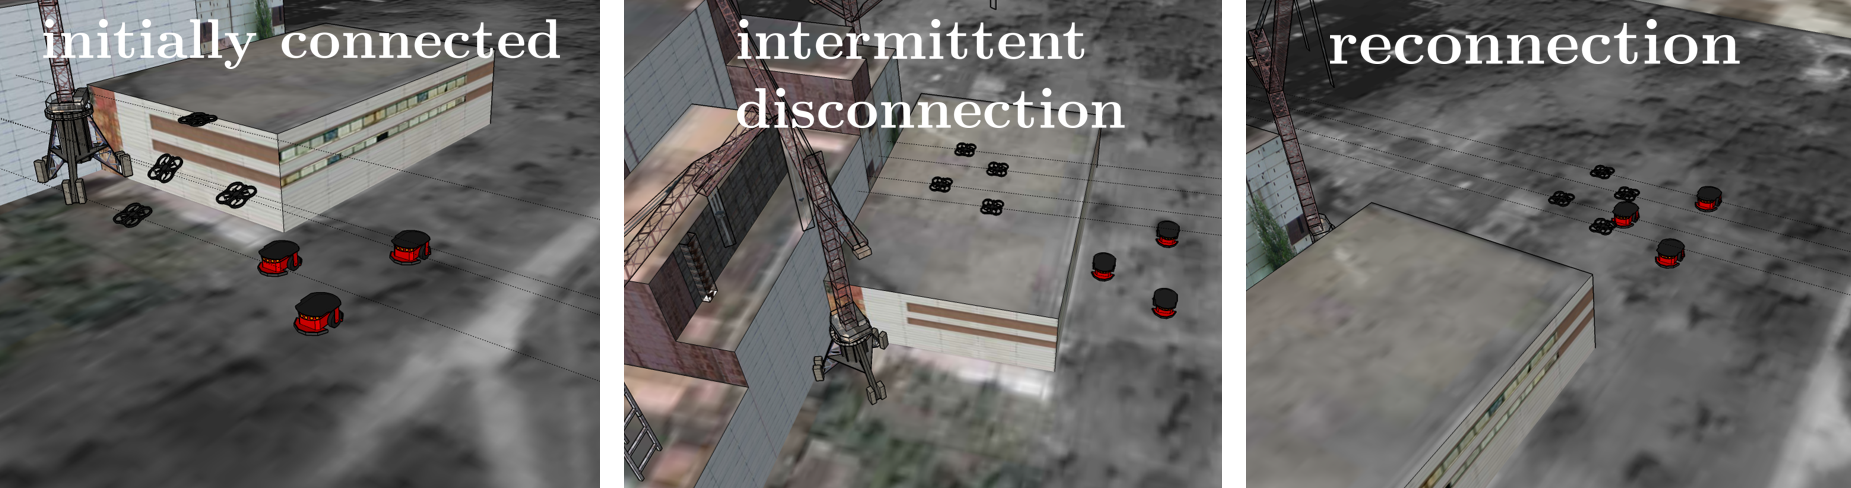
\includegraphics[width=1\linewidth]{scenario_robots3.png}
				\label{fig:diffusion2}
			\end{figure}
		\end{column}
		
		\begin{column}{.33\textwidth}
			\begin{figure}
				\centering
				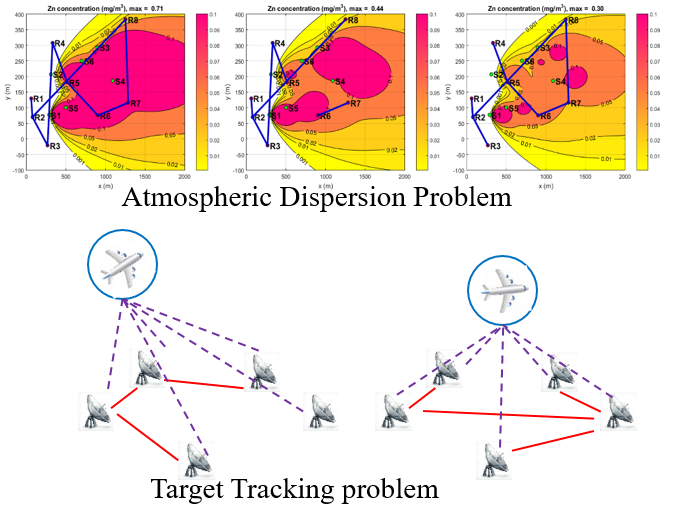
\includegraphics[width=1\linewidth]{target_tracking}
			\end{figure}
		\end{column}
	\end{columns}
\vspace{-1.3cm}
%	
%		\begin{column}{.33\textwidth}
%			\begin{figure}
%				\centering
%				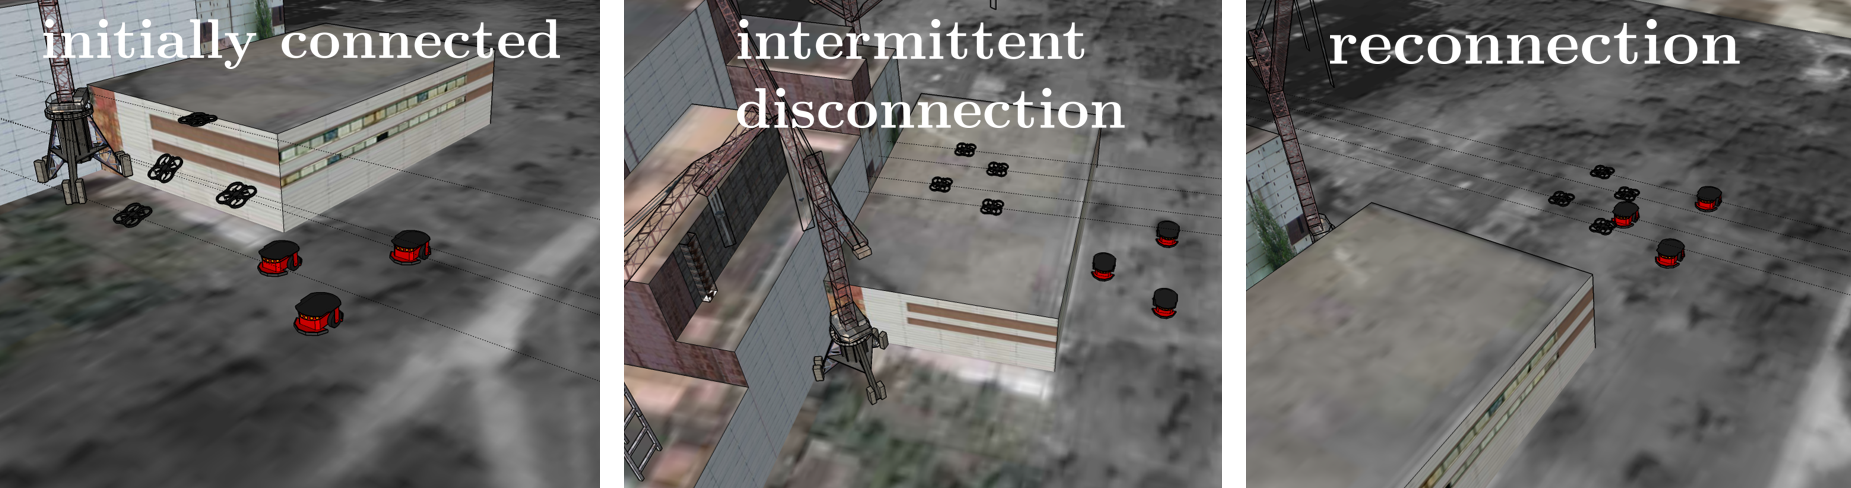
\includegraphics[width=1\linewidth]{scenario_robots3.png}
%				\label{fig:diffusion}
%			\end{figure}
%		\end{column}
%			\begin{column}{.33\textwidth}
%				\begin{figure}
%					\centering
%					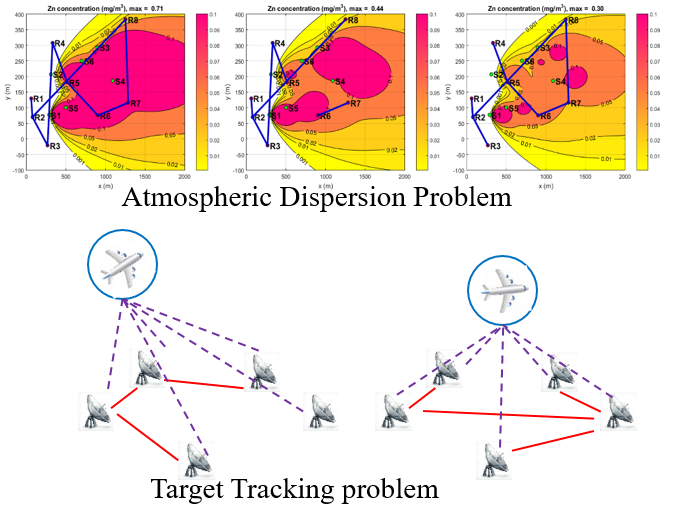
\includegraphics[width=1\linewidth]{target_tracking}
%					\label{fig:diffusion}
%				\end{figure}
%			\end{column}

\end{center}
%\vspace{0.3cm}
\begin{columns}
	\begin{column}{.33\textwidth}
		\begin{figure}
			\centering
			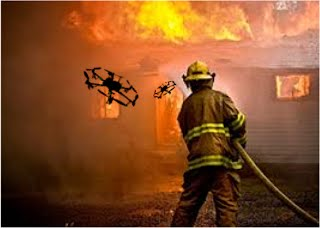
\includegraphics[width=1\linewidth]{ff_drones.jpg}
			\caption*{\tiny source: \href{https://sites.google.com/a/ncsu.edu/firefighting-drone-challenge/}{\tiny https://sites.google.com/a/ncsu.edu/firefighting-drone-challenge/}}
			\label{fig:diffusion}
		\end{figure}
	\end{column}
	
	\begin{column}{.33\textwidth}
		
\includegraphics[width=1\linewidth]{objective.png}
%\includesvg{objectives}
	\end{column}	
	
	\begin{column}{.34\textwidth}
		\begin{figure}
			\centering
			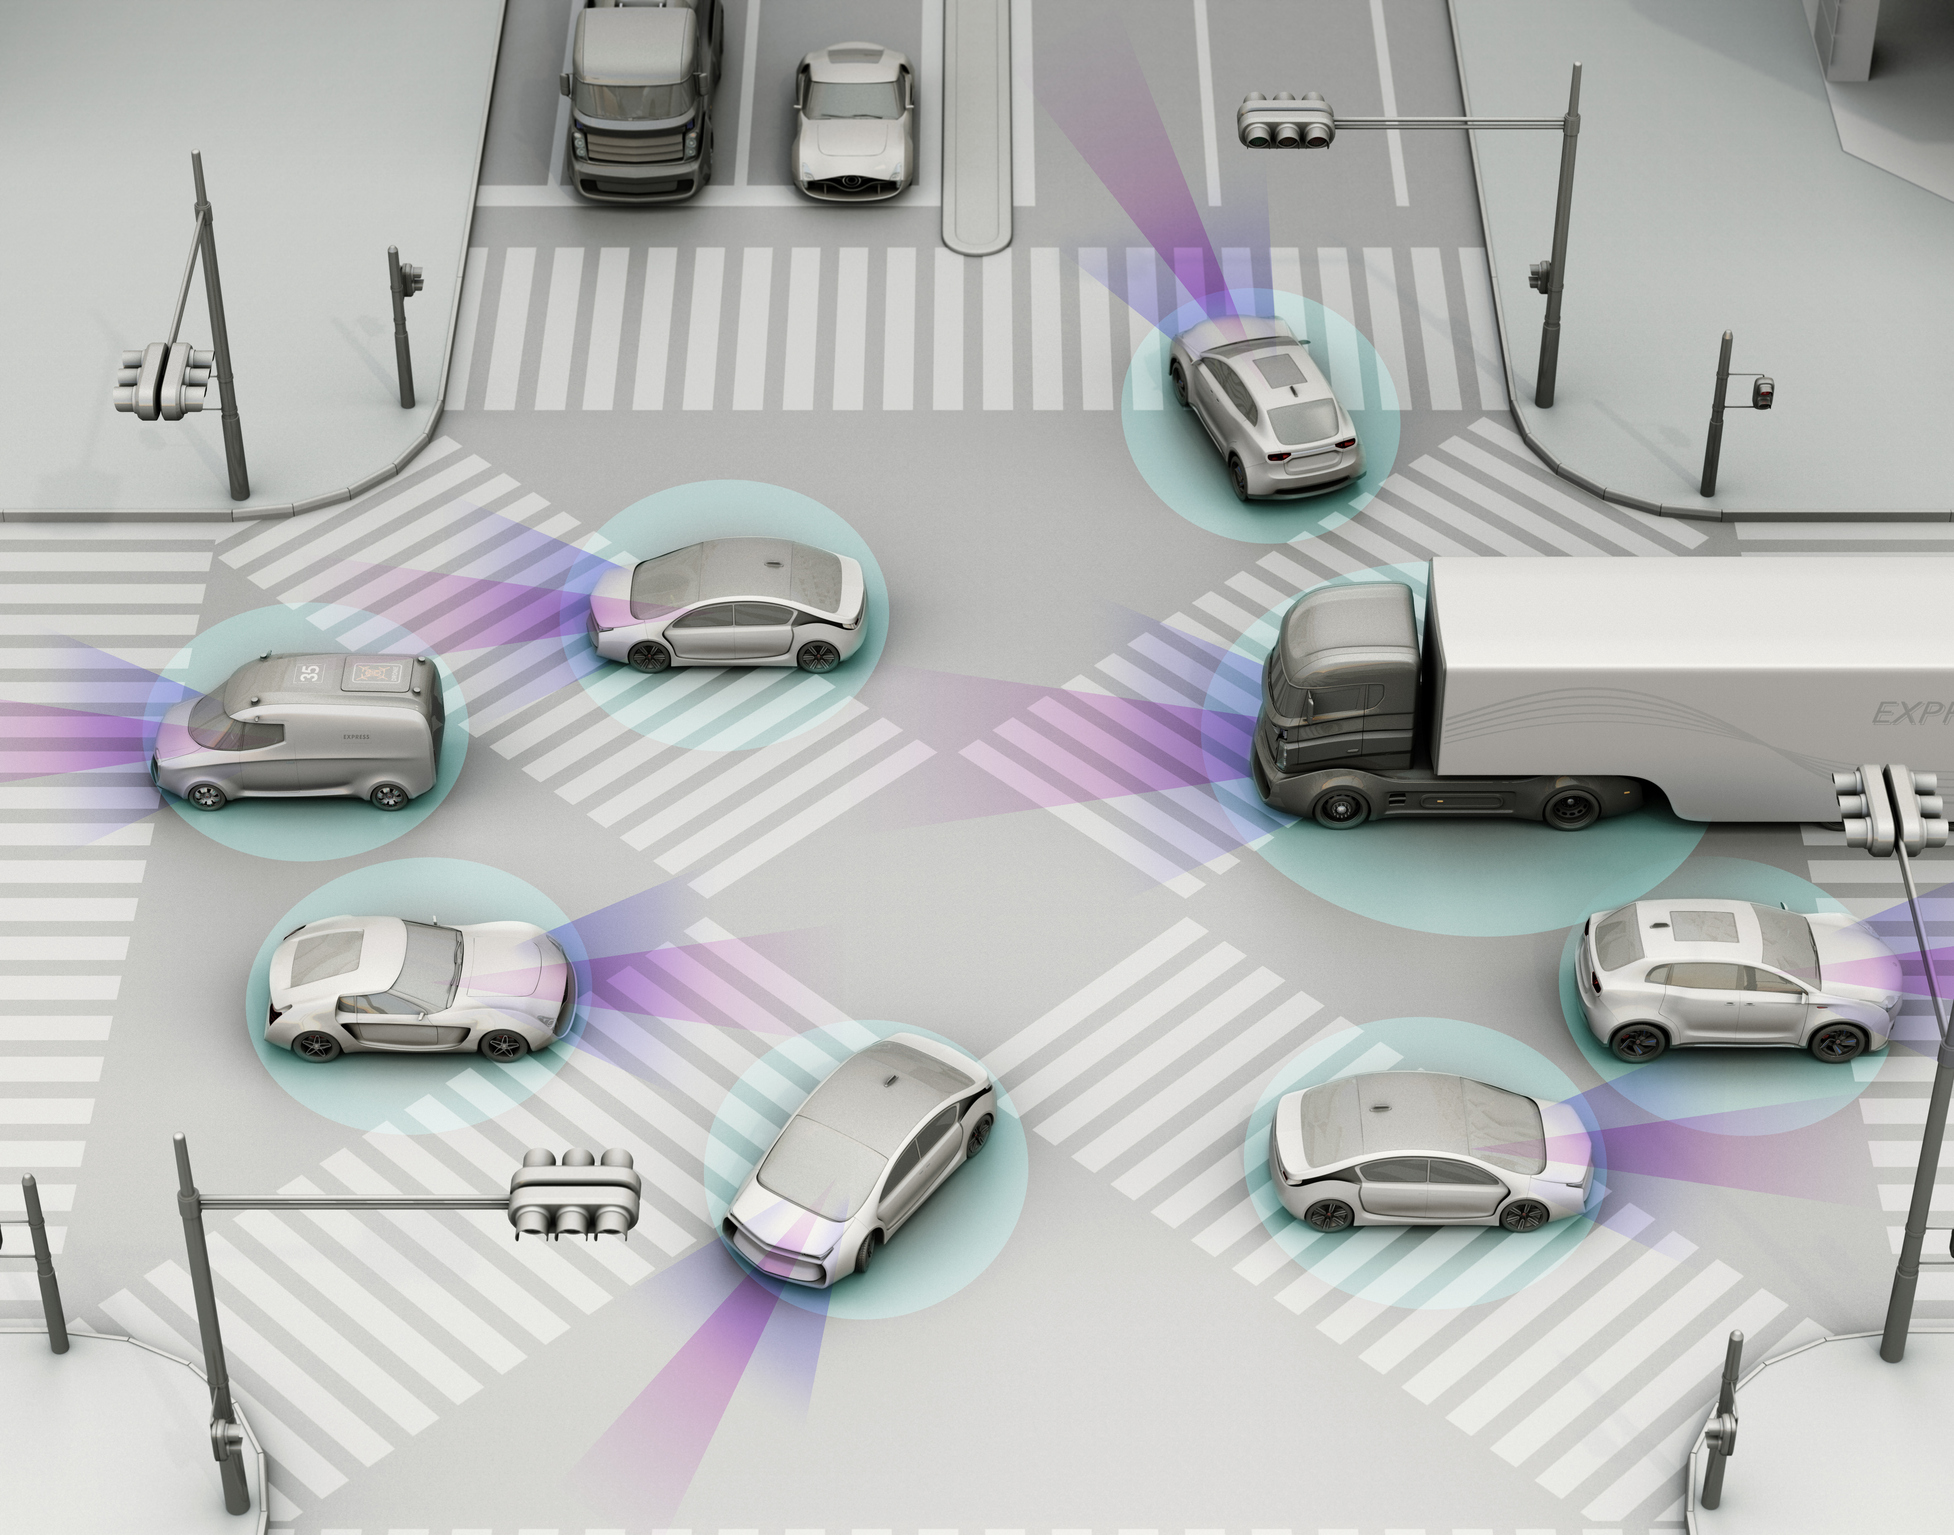
\includegraphics[width=1\linewidth]{sdc.jpg}
			\caption*{\tiny source: \href{http://statescoop.com/self-driving-in-north-dakota-new-research-to-target-data-privacy-safety}{\tiny http://statescoop.com/self-driving-in-north-dakota-new-research-to-target-data-privacy-safety}}
		\end{figure}
	\end{column}
\end{columns}




%
%\begin{figure}
%	\centering
%	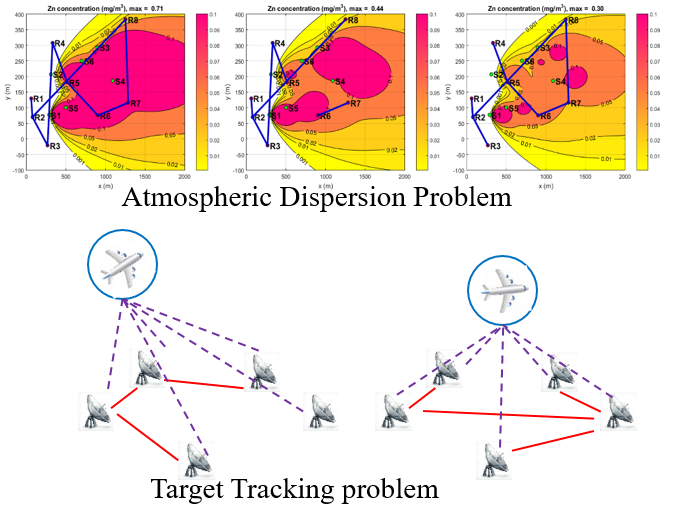
\includegraphics[width=0.5\linewidth]{target_tracking}
%	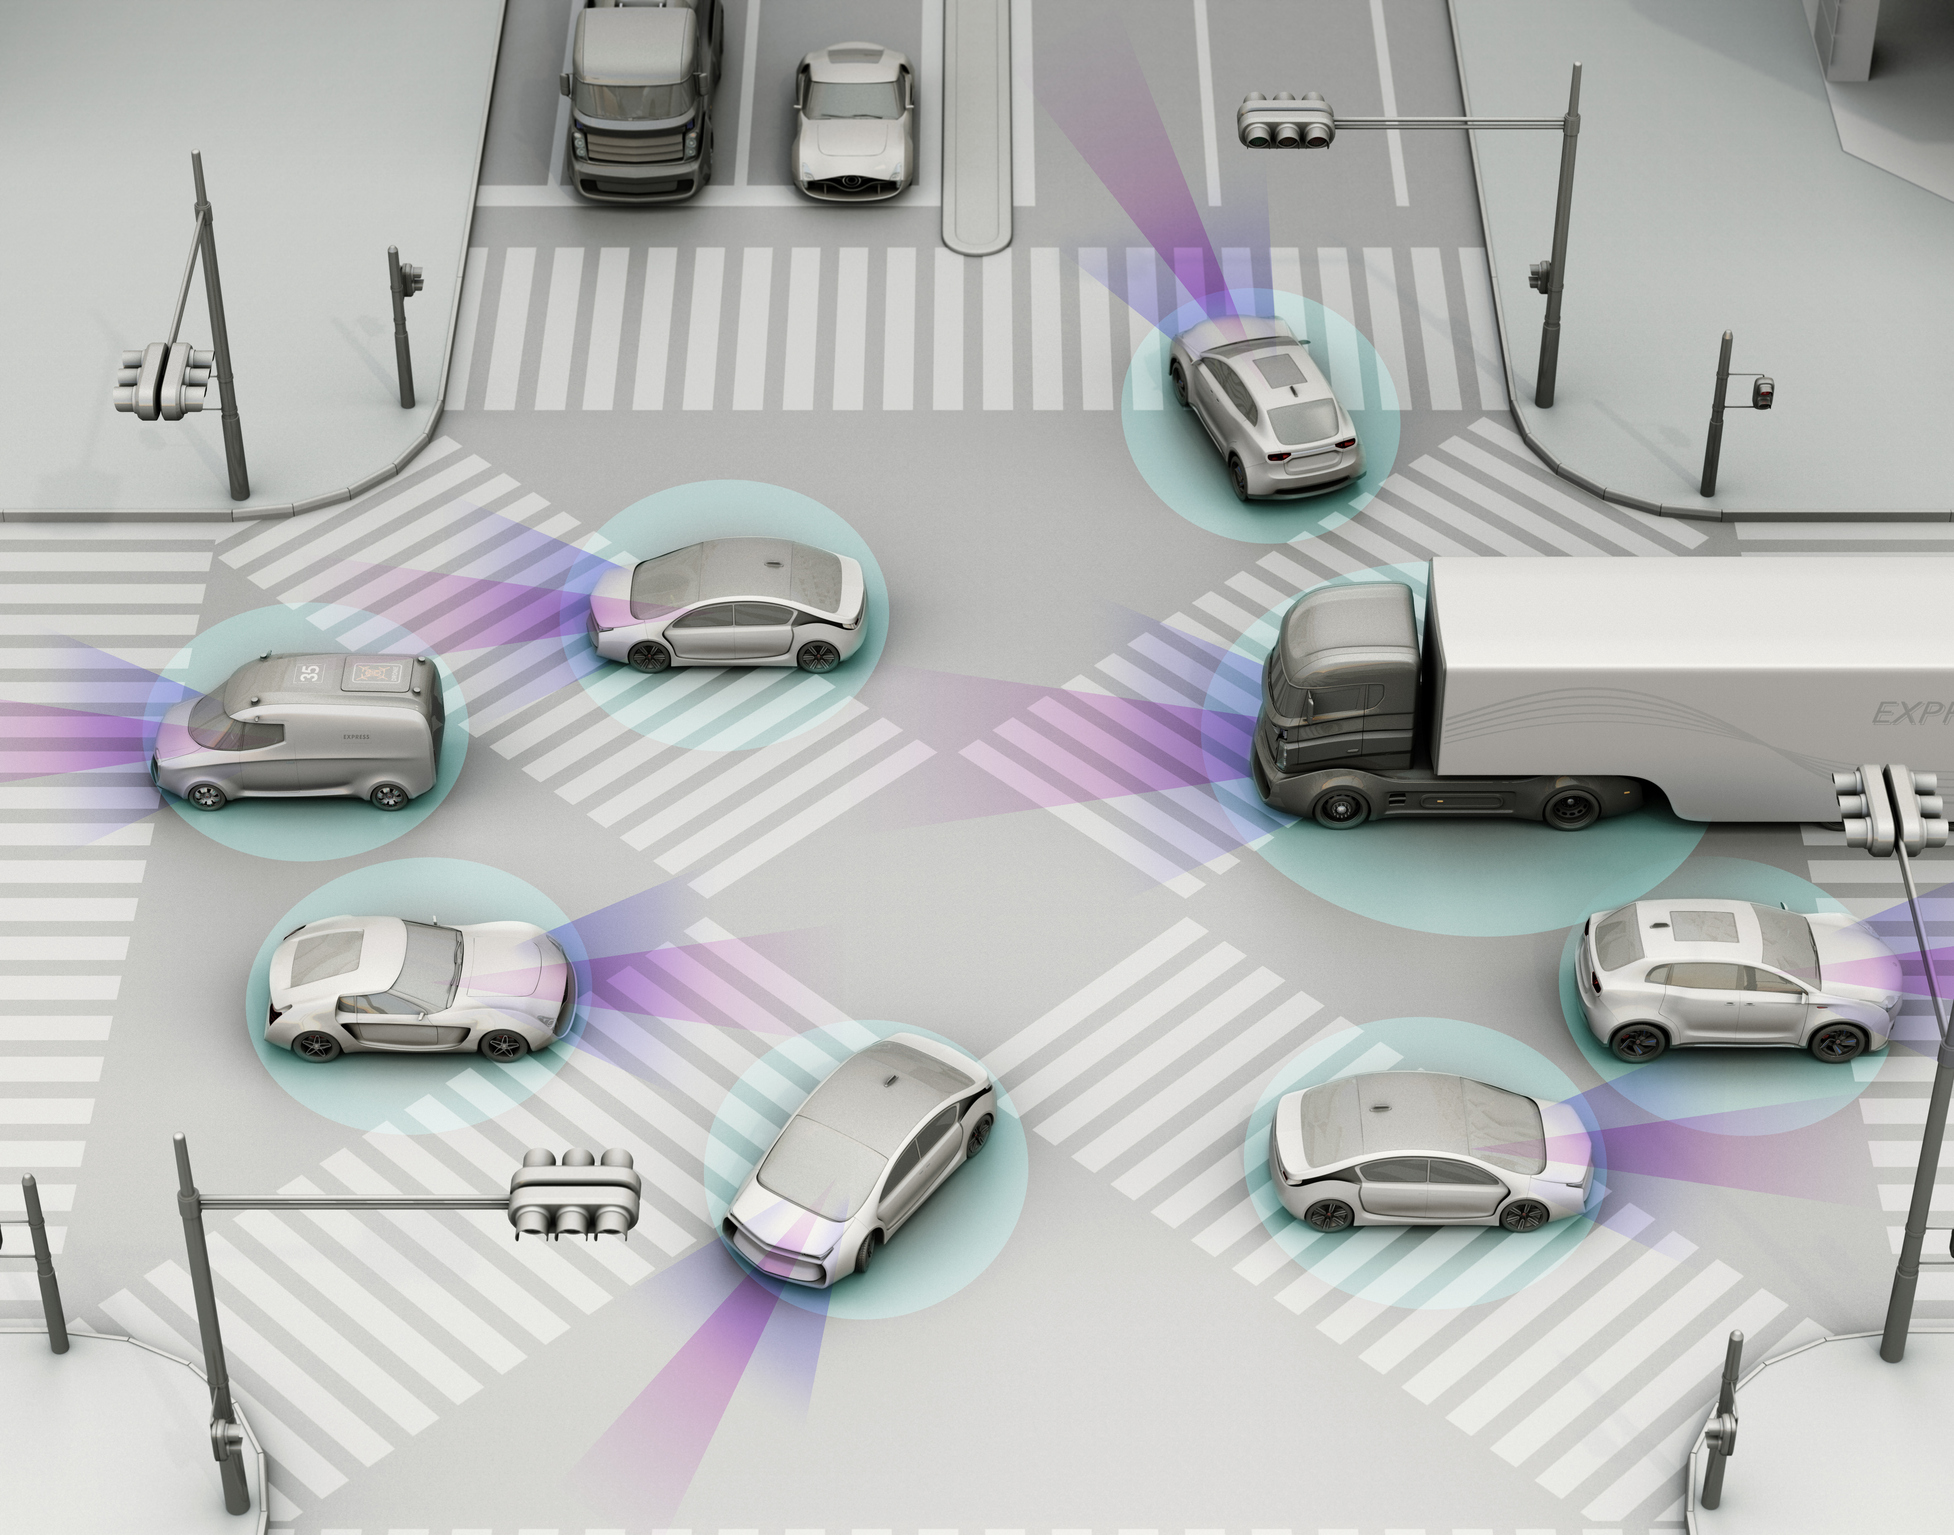
\includegraphics[width=0.5\linewidth]{sdc.jpg}
%	\caption{source}
%	\label{fig:target_tracking}
%\end{figure}
%\begin{figure}
%	\centering
%	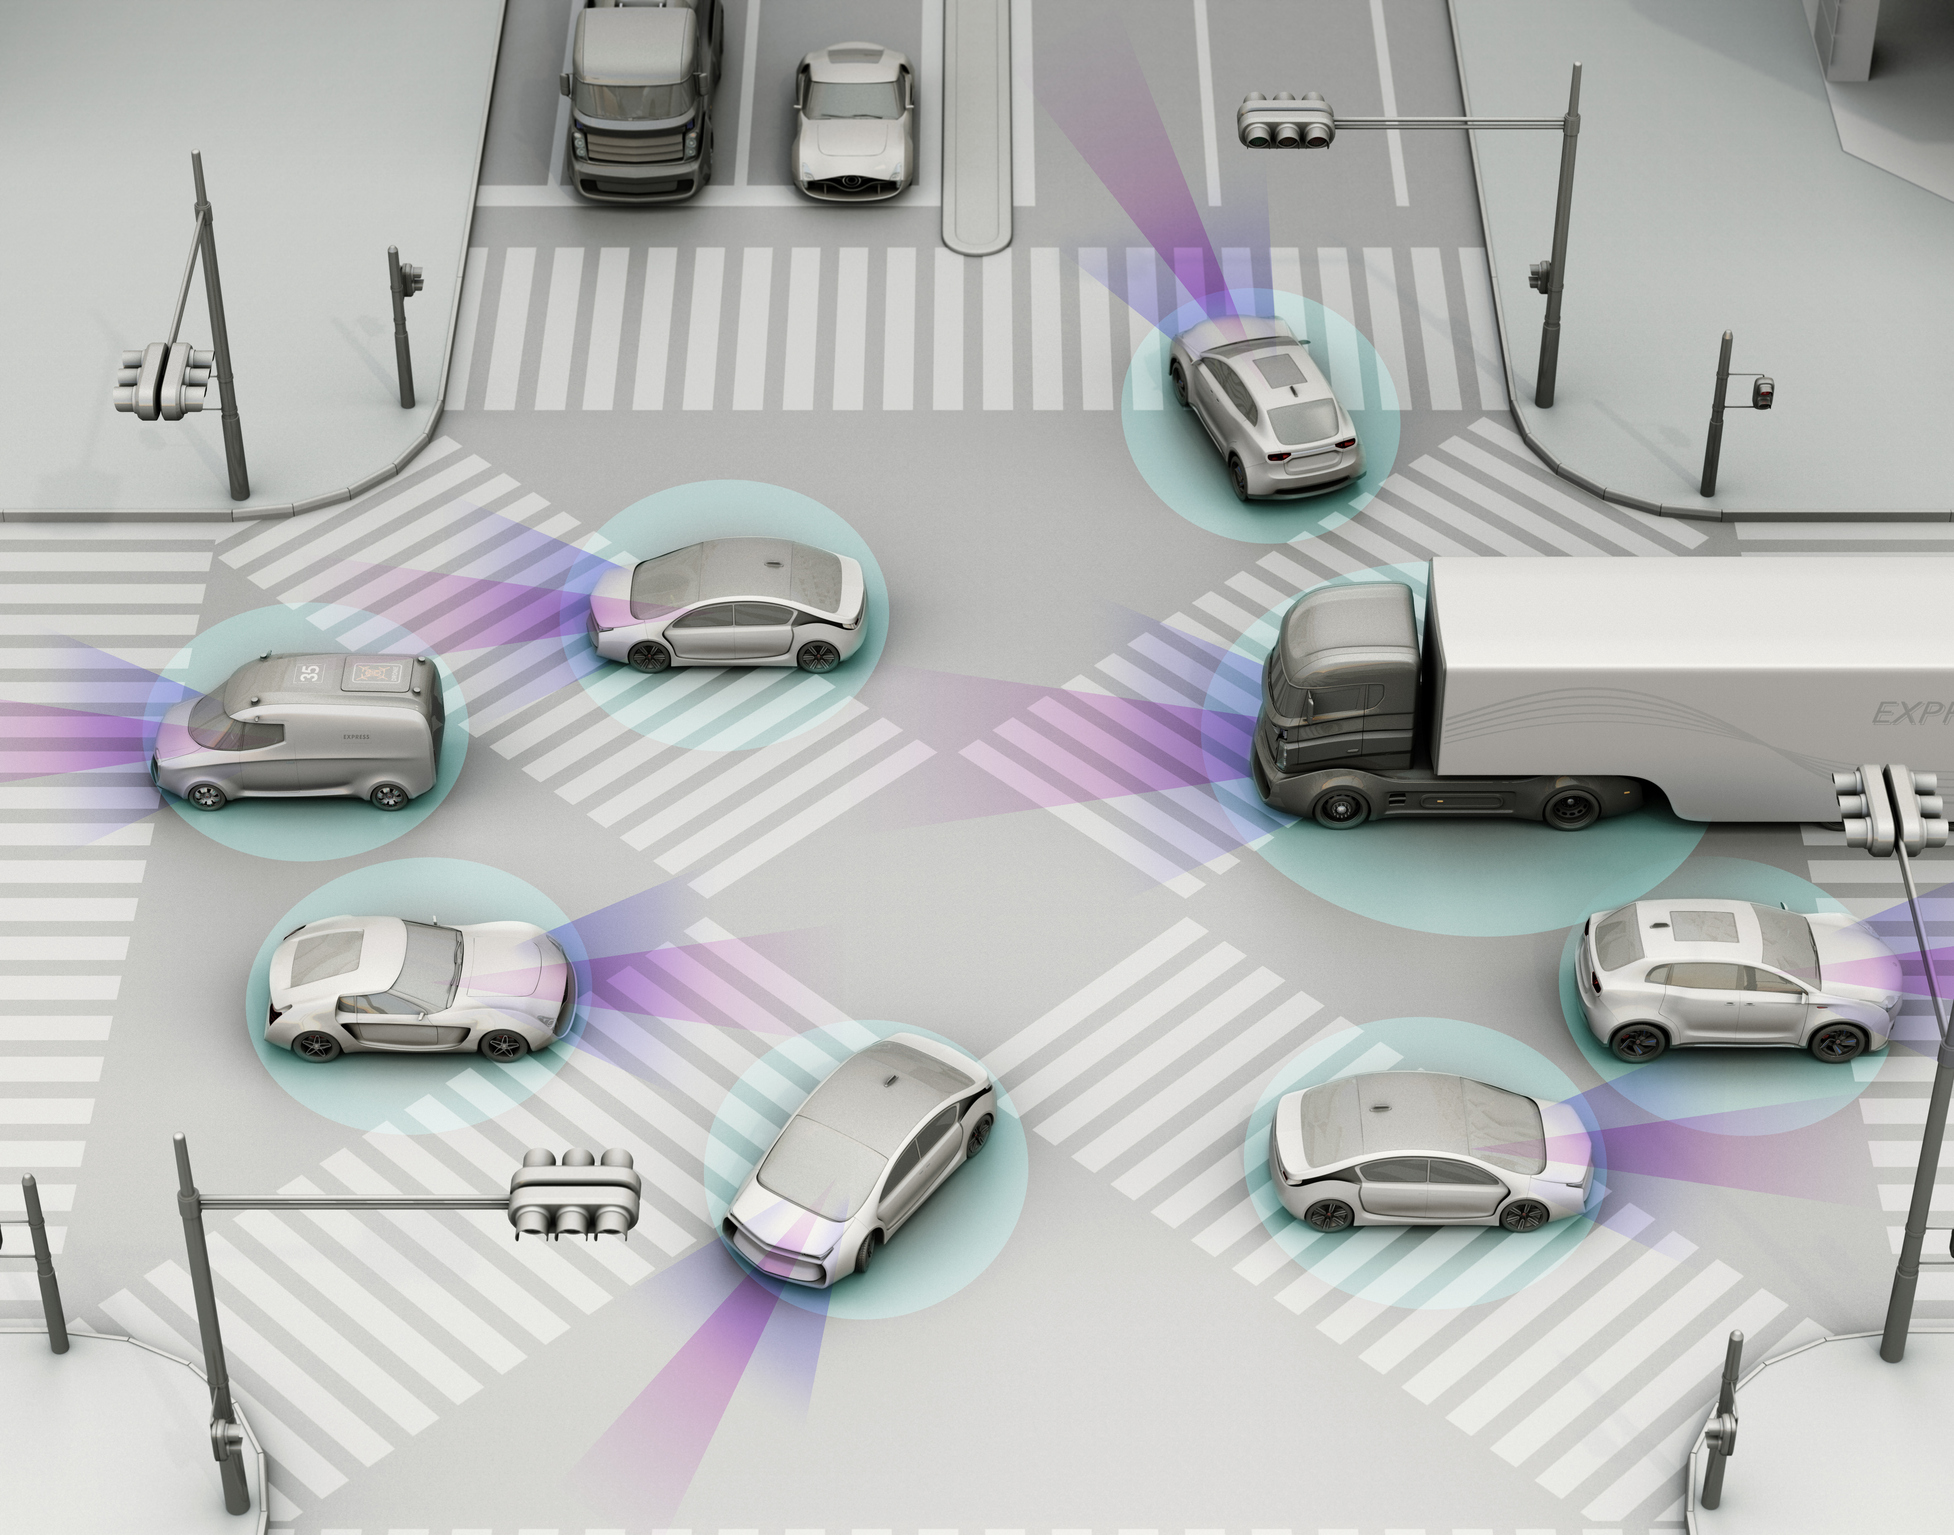
\includegraphics[width=0.6\linewidth]{sdc.jpg}
%	\label{fig:self_driving_cars}
%\end{figure}
\end{frame}
\begin{frame}{Synopsis}
			\begin{figure}
				\centering
	 			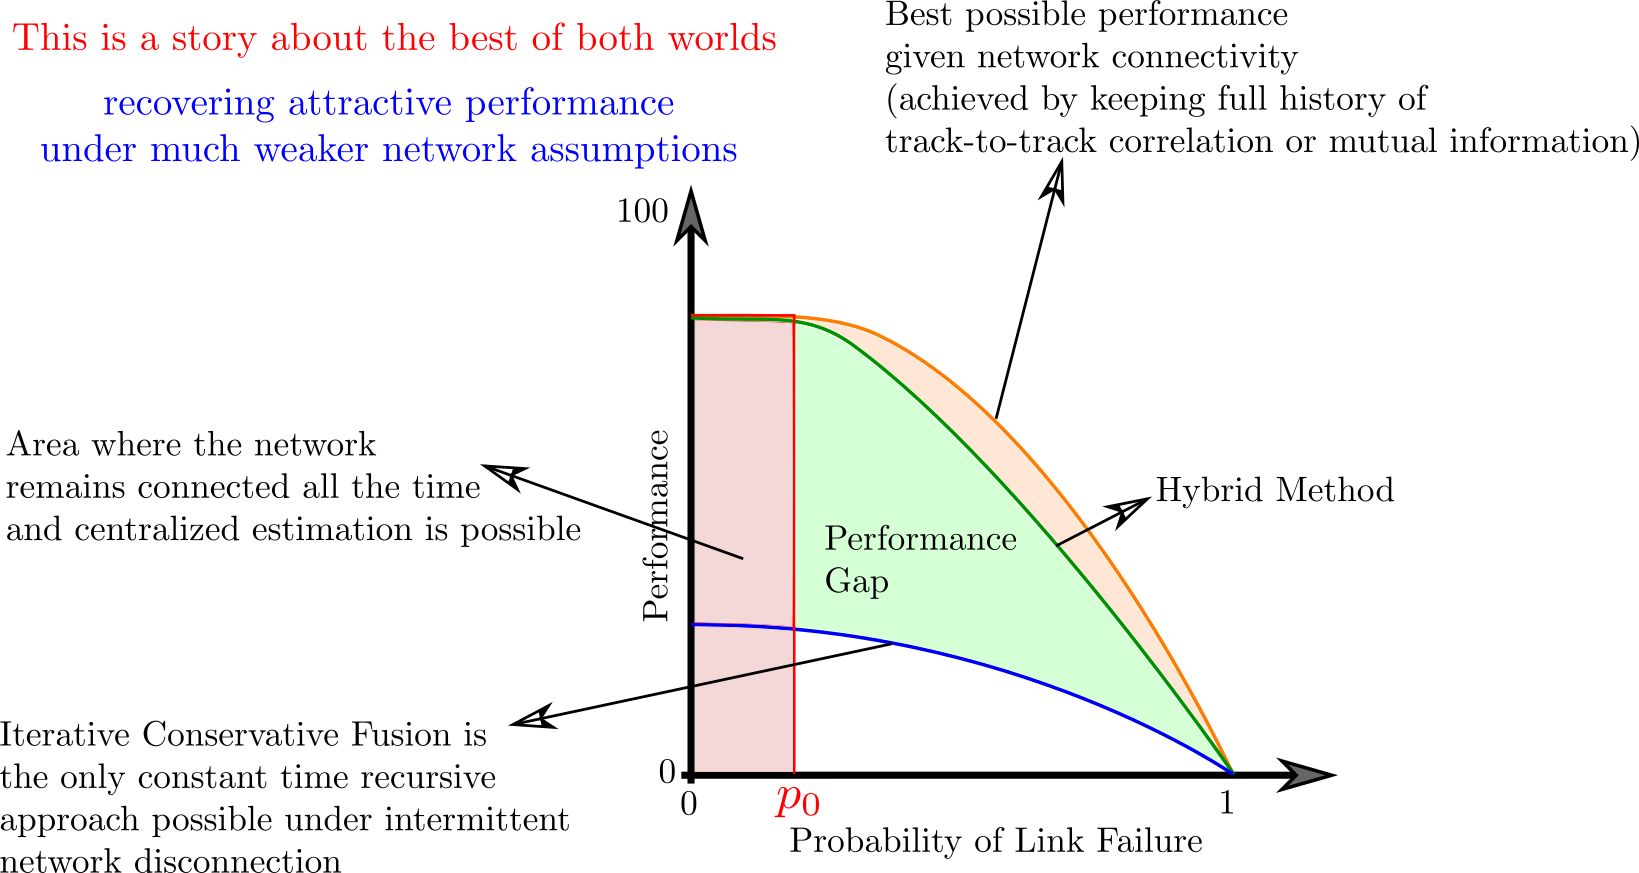
\includegraphics[width=1\linewidth]{synopsis5.png}
			\end{figure}
	

\end{frame}
\begin{frame}{Bayesian Estimation}
	
				\begin{align*}
				& {\color{brown}\overbrace{\textstyle \pr(\XX[]{k}{}|\{\zz{k}{i}\}^{i\in\bIn}_{k\in\bIk}) }^{posterior}}  = \frac{1}{\eta}  
				{\color{blue}\overbrace{\pr(\{\zz{k}{i}\}^{i\in\bIn}| \XX[]{k}{})}^{\textit{observation model}\textbf{}}}
				{\color{red}\overbrace{\pr(\XX[]{k}{}|\{\zz{k}{i}\}^{i\in\bIn}_{k\in\bIkk})}^{prediction}} \\
				&\textstyle = \frac{1}{\eta}\prod_{i=1}^{n} 
				{\color{orange}\overbrace{\pr(\vect{z}_{k}^i | \XX[]{k}{})}^{\textit{agent obs. mdl.}}} \int {\color{cyan}\overbrace{\pr(\vect{X}_{k} | \XX[]{k-1}{})}^{\textit{motion model}}} {\color{brown}\overbrace{\pr(\XX[]{k-1}{}|\{\zz{k}{i}\}^{i\in\bIn}_{k\in\bIkk})}^{prior}}d\XX[]{k-1}.
				\end{align*}	
	\centering
	\begin{columns}
		\begin{column}{.48\textwidth}
%					\begin{figure}
%						\centering
%						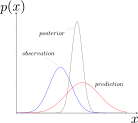
\includegraphics[width=0.7\linewidth]{estimate.png}
%					\end{figure}
\begin{tikzpicture}[scale=0.5]
\begin{axis}[every axis plot post/.append style={
	mark=none,domain=-2:3,samples=50,smooth}, % All plots: from -2:2, 50 samples, smooth, no marks
axis x line=bottom, % no box around the plot, only x and y axis
axis y line=left, % the * suppresses the arrow tips
enlargelimits=upper,
yticklabels={,,},
xticklabels={,,}] % extend the axes a bit to the right and top
\addplot {gauss(0,0.5)};
\addplot {gauss(1,0.75)};
\addplot {gauss(0.75,0.25)};
\node at (axis cs:0, 0.7978845608) [pin=110: $observation$] {};
\node at (axis cs:1, 0.4978845608) [pin=0: $prediction$] {};
\node at (axis cs:0.75, 1.4978845608) [pin=190: $posterior$] {};
\end{axis}
\end{tikzpicture}
		\end{column}
		
		\begin{column}{.48\textwidth}
			$k$ : time step
			
			$\XX[]{k}{}$ : state (ex. position of a robot)
			
			$\zz{k}{i}$ : observation by agent $i$ \\(ex. distance to wall)
			
			 $\bIk = \{1,2,\cdots,k\}$ index set
			
			

		\end{column}
				
	\end{columns}
			
	
	
	
	
%	\begin{columns}
%		\begin{column}{.48\textwidth}
%				\centering
%				\begin{tikzpicture}[scale=0.5]
%				\begin{axis}[every axis plot post/.append style={
%					mark=none,domain=-2:3,samples=50,smooth}, % All plots: from -2:2, 50 samples, smooth, no marks
%				axis x line=bottom, % no box around the plot, only x and y axis
%				axis y line=left, % the * suppresses the arrow tips
%				enlargelimits=upper,
%				yticklabels={,,},
%				xticklabels={,,}] % extend the axes a bit to the right and top
%				\addplot {gauss(0,0.5)};
%				\addplot {gauss(1,0.75)};
%				\addplot {gauss(0.75,0.25)};
%				\node at (axis cs:0, 0.7978845608) [pin=150: $observation$] {};
%				\node at (axis cs:1, 0.4978845608) [pin=0: $prediction$] {};
%				\node at (axis cs:0.75, 1.4978845608) [pin=190: $posterior$] {};
%				\end{axis}
%				\end{tikzpicture}
%		\end{column}
%		
%		\begin{column}{.48\textwidth}
%		\begin{align*}
%		& {\color{brown}\overbrace{\textstyle \pr(\XX[]{k}{}|\{\zz{k}{i}\}^{i\in\bIn}_{k\in\bIk}) }^{posterior}}  = \frac{1}{\eta}  
%		{\color{blue}\overbrace{\pr(\{\zz{k}{i}\}^{i\in\bIn}| \XX[]{k}{})}^{\textit{observation model}\textbf{}}}
%		{\color{red}\overbrace{\pr(\XX[]{k}{}|\{\zz{k}{i}\}^{i\in\bIn}_{k\in\bIkk})}^{prediction}} \\
%		&\textstyle = \frac{1}{\eta}\prod_{i=1}^{n} 
%		{\color{orange}\overbrace{\pr(\vect{z}_{k}^i | \XX[]{k}{})}^{\textit{agent obs. mdl.}}} \int {\color{cyan}\overbrace{\pr(\vect{X}_{k} | \XX[]{k-1}{})}^{\textit{motion model}}} {\color{brown}\overbrace{\pr(\XX[]{k-1}{}|\{\zz{k}{i}\}^{i\in\bIn}_{k\in\bIkk})}^{prior}}d\XX[]{k-1}.
%		\end{align*}
%		\end{column}
%	\end{columns}
\end{frame}
	
	
	
	

%\pgfplotsset{%
%	colormap={whitered}{color(0cm)=(white);
%		color(1cm)=(orange!75!red)}
%}
%\pgfplotsset{%
%	colormap={bluered}{color(0cm)=(white);
%		color(1cm)=(blue!75!red)}
%}
%
%\begin{tikzpicture}[
%scale = 0.2,
%declare function = {mu1=1;},
%declare function = {mu2=2;},
%declare function = {sigma1=0.5;},
%declare function = {sigma2=1;},
%declare function = {normal(\m,\s)=1/(2*\s*sqrt(pi))*exp(-(x-\m)^2/(2*\s^2));},
%declare function = {bivar(\ma,\sa,\mb,\sb)=
%	1/(2*pi*\sa*\sb) * exp(-((x-\ma)^2/\sa^2 + (y-\mb)^2/\sb^2))/2;}]
%\begin{axis}[
%colormap name  = whitered,
%width          = 15cm,
%view           = {45}{65},
%enlargelimits  = false,
%domain         = -1:4,
%y domain       = -1:4,
%samples        = 10,
%xlabel         = $x_1$,
%ylabel         = $x_2$,
%zlabel         = {$P$},
%colorbar,
%colorbar style = {
%	at     = {(1,0)},
%	anchor = south west,
%	height = 0.25*\pgfkeysvalueof{/pgfplots/parent axis height},
%	title  = {$P(x_1,x_2)$}
%}
%]
%\addplot3[surf,opacity = 0.8] {bivar(mu1,sigma1,mu2,sigma2)};
%\addplot3[opacity = 0.1] {bivar(mu2,sigma2,mu1,sigma1)};
%\addplot3[
%surf,
%opacity=0.8,
%samples=50, samples y=30,
%colormap/bluered,
%domain=-1:4,domain y=-1:4
%%z buffer=sort,
%]
%{((x+sin(deg(x)))^2};
%
%(x,4,{normal(mu1,sigma1)});
%\addplot3 [domain=-1:4,samples=31, samples y=0, thick, smooth]
%(-1,x,{normal(mu2,sigma2)});
%
%\draw [black!50] (axis cs:-1,0,0) -- (axis cs:4,0,0);
%\draw [black!50] (axis cs:0,-1,0) -- (axis cs:0,4,0);
%
%\node at (axis cs:-1,1,0.18) [pin=165:$P(x_1)$] {};
%\node at (axis cs:1.5,4,0.32) [pin=-15:$P(x_2)$] {};
%\end{axis}
%\end{tikzpicture}


\section{Distributed State Estimation Preliminaries} 
\begin{frame}{Estimation on Sensor Networks}
\label{subsec:Preliminaries}
{\color{red} Recursive State Estimation}
 is the process of recursively computing the posterior probability of a random dynamic process $\XX[]{k}{}$ conditioned on a sequence of measurements $\{\zz{k}{i}\}^{i\in\bIn}_{k\in\bIk}$. 
	\begin{align*}
	& {\color{brown}\overbrace{\textstyle \pr(\XX[]{k}{}|\{\zz{k}{i}\}^{i\in\bIn}_{k\in\bIk}) }^{posterior}}  = \frac{1}{\eta}  
	{\color{blue}\overbrace{\pr(\{\zz{k}{i}\}^{i\in\bIn}| \XX[]{k}{})}^{\textit{observation model}\textbf{}}}
			{\color{red}\overbrace{\pr(\XX[]{k}{}|\{\zz{k}{i}\}^{i\in\bIn}_{k\in\bIkk})}^{prediction}} \\
	&\textstyle = \frac{1}{\eta}\prod_{i=1}^{n} 
	{\color{orange}\overbrace{\pr(\vect{z}_{k}^i | \XX[]{k}{})}^{\textit{agent obs. mdl.}}} \int {\color{cyan}\overbrace{\pr(\vect{X}_{k} | \XX[]{k-1}{})}^{\textit{motion model}}} {\color{brown}\overbrace{\pr(\XX[]{k-1}{}|\{\zz{k}{i}\}^{i\in\bIn}_{k\in\bIkk})}^{prior}}d\XX[]{k-1}.
	\end{align*}
\vspace{-0.9cm}
\begin{columns}
	\begin{column}{.48\textwidth}
		\begin{figure}
			\centering
			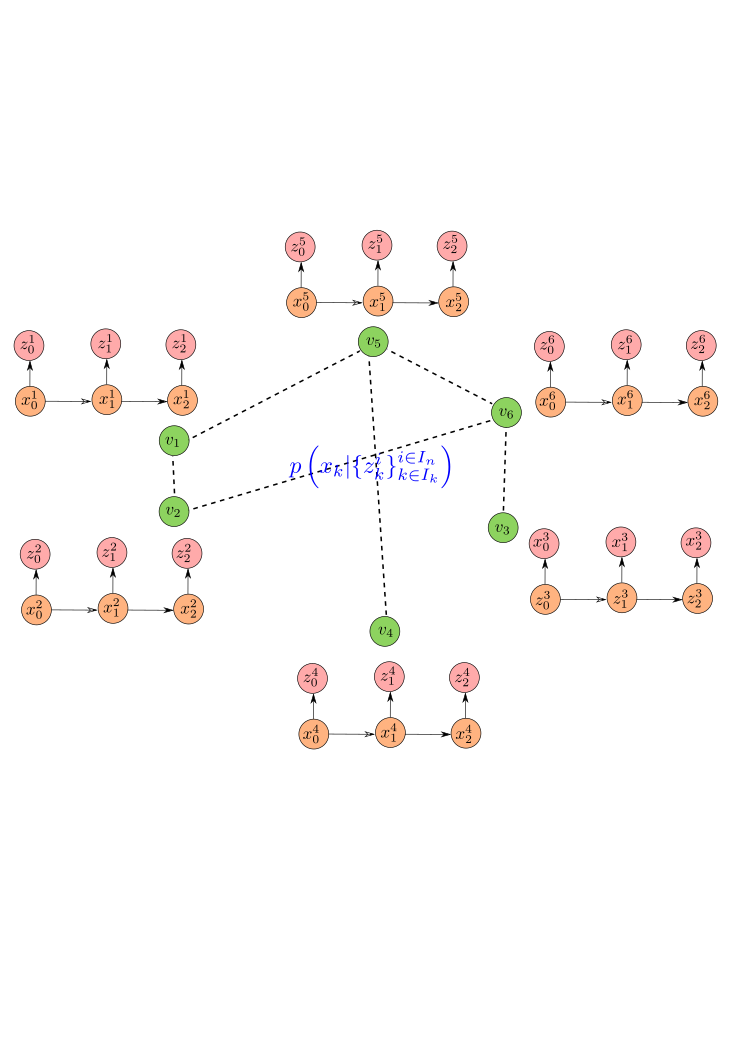
\includegraphics[trim={0cm 8cm 0cm 8cm},clip,width=0.8\linewidth]{drawing.png}
			\vspace{-0.7cm}
			\caption*{Distributed}
			\label{fig:fu}
		\end{figure}
	\end{column}
	
	\begin{column}{.48\textwidth}
		\begin{figure}
			\centering
			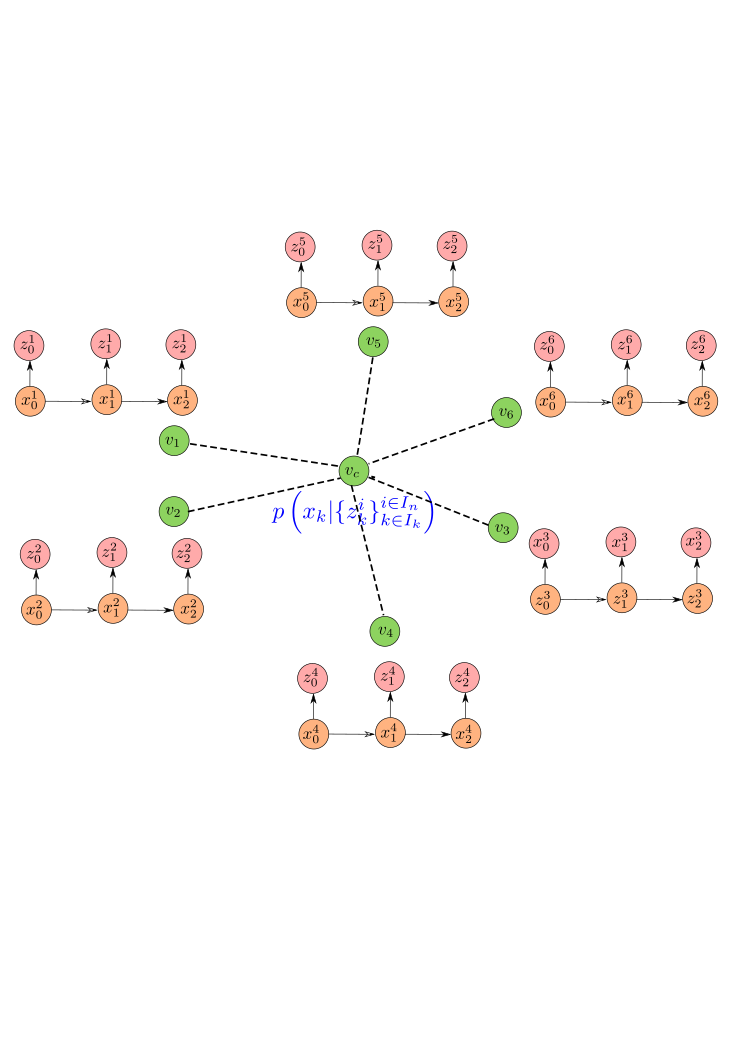
\includegraphics[trim={0cm 8cm 0 8cm},clip,width=0.8\linewidth]{drawing2.png}
			\vspace{-0.7cm}
			\caption*{Centralized}
		\end{figure}
	\end{column}
\end{columns}
\end{frame}

\begin{frame}{Distributed State Estimation (DSE)}
	
{\color{red} Why Distributed State Estimation?} 

\begin{itemize}
\item[$\bullet$] {Difficulty of centralized estimator implementation due to bandwidth and energy constraints}
{\item[$\bullet$] scalability}
\item[$\bullet$] modularity
\item[$\bullet$] robustness to network failure
\end{itemize}

  \begin{table}[h]
 	\centering
 	\resizebox{0.9\textwidth}{!}{\begin{tabular}{||p{6cm} |p{7cm} | p{7cm}||} 
 		\hline\hline
 		 {\color{blue}state} & static {\color{olive} \citep{xiao2005scheme}} & dynamic {\color{olive}\citep{5509143}}\\ 
 		  		\hline\hline
 		 {\color{blue}transition model} & linear  {\color{olive}\citep{olfati2005distributed}} & non-linear {\color{olive}\citep{battistelli2014parallel}} \\
 		  		\hline\hline
 		 {\color{blue}topology of the network} & always connected {\color{olive}\citep{battistelli2014parallel}} & intermittent disconnection {\color{olive}\citep{tamjidi2016unifying,xiao2005scheme}} \\
 		  		\hline\hline
 		 {\color{blue}knowledge of the network topology} & global{\color{olive}\citep{xiao2005scheme}} & local {\color{olive}\citep{tamjidi2016unifying,xiao2005scheme,battistelli2014parallel}} \\
 		  		  		\hline\hline
 		 {\color{blue}treatment of  mutual information} & channel filter  {\color{olive}\citep{durrant2001data}} & avoid double counting {\color{olive}\citep{wang_distr_CI,hu2012diffusion}}\\ 
 		  		  		  		\hline\hline 
 	 {\color{blue}noise} & gaussian  {\color{olive}\citep{olfati2005distributed,cattivelli2010diffusion}} & non-gaussian {\color{olive}\citep{lin_dist_part_filter_2014}}\\ 
 	 \hline\hline 		  		  		  		
 		  		  		  		
 		 	\end{tabular}}
 	\caption{Categories of Methods}
 	\label{table:1}
 \end{table}
 \vspace{-0.5cm}
The DSE algorithms  {\color{red}are not guaranteed to match the performance of the centralized estimator} all the time
\end{frame}

\section{Hidden Markov Model and Network Topology}
\begin{frame}{Hidden Markov Model}
	
			\begin{exampleblock}{}
	\subsubsection*{Hidden Markov Model} Consider a finite state hidden markov model (HMM)   with the following specification:
	$n_s$ possible states {\color{red}$\mathcal{X} = \{S_1,\cdots,S_{n_s}\} $ }and  $n_z$ possible observation symbols listed as {\color{red} $\mathcal{Z} = \{O_1,\cdots,O_{n_z}\}$}.
	The random variables {\color{red}$\vect{X}_k \in \mathcal{X} $} and {\color{red}$ \vect{Z}_k^i \in \mathcal{Z} $} represent the state and observation made by agent $i$ at step $ k $, respectively. The realizations of those random variables at step $k$ is denoted as $\vect{x}_k$ and $\vect{z}_k^i$.    
		{\color{blue}
			\begin{align}
			\pi_{k-1}&\triangleq \pr\left(\XX[]{k-1}{}|\{\zz{k}{i}\}^{i\in\bIn}_{k\in\bIkk}\right),\nonumber\\
			\tilde{\pi}_{k}&\triangleq \pr\left(\XX[]{k}{}|\{\zz{k}{i}\}^{i\in\bIn}_{k\in\bIkk}{}\right),\nonumber\\
			\pi_{k}&\triangleq \pr\left(\XX[]{k}{}|\{\zz{k}{i}\}^{i\in\bIn}_{k\in\bIk}\right),\nonumber
			\end{align}}
		\end{exampleblock}
\end{frame}
\begin{frame}{Hidden Markov Model}
\begin{columns}
		\begin{column}{.33\textwidth}
			\begin{figure}
				\centering
				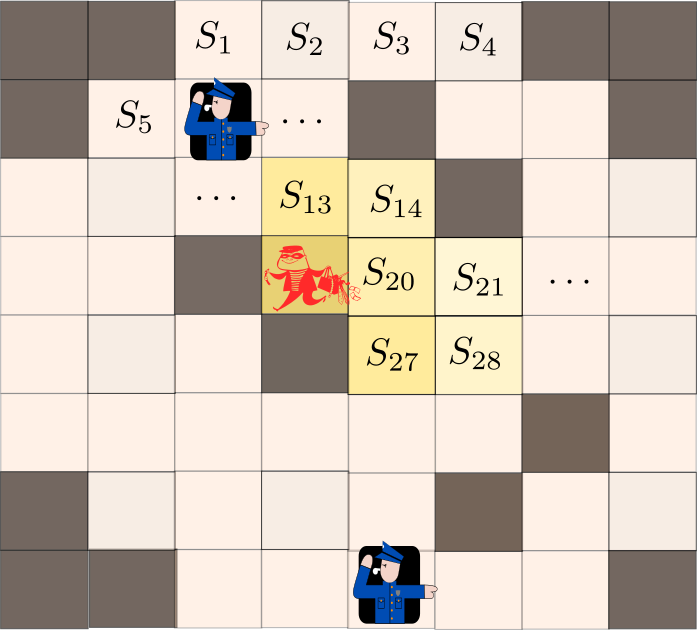
\includegraphics[width=0.9\linewidth]{prior2.png}
				\vspace{-10pt}
				\caption*{\tiny prior}

				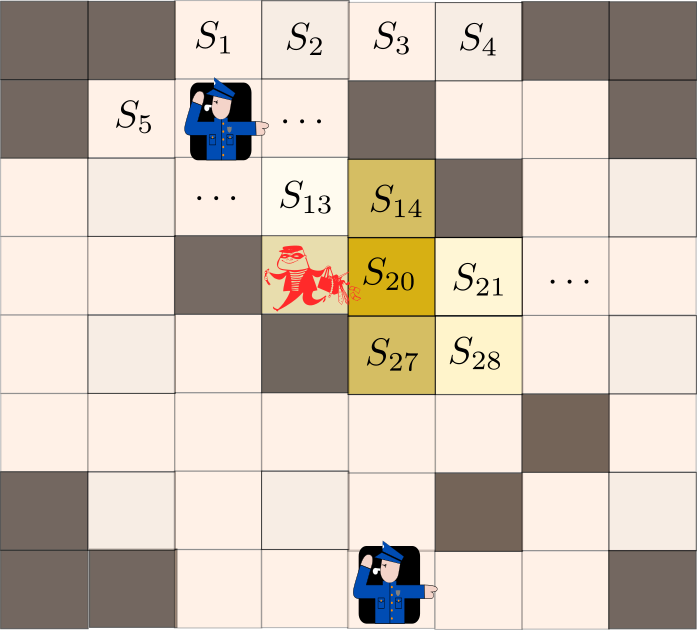
\includegraphics[width=0.9\linewidth]{motion.png}
				\vspace{-10pt}
				\caption*{\tiny motion model}
			\end{figure}
		\end{column}
	\begin{column}{.33\textwidth}
		\begin{figure}
			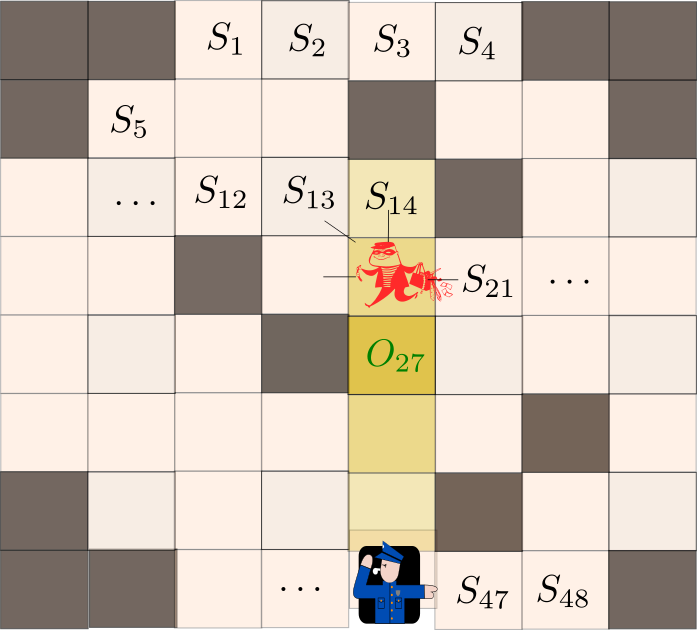
\includegraphics[width=0.9\linewidth]{observation1.png}
			\vspace{-10pt}
			\caption*{\tiny observation 1}

			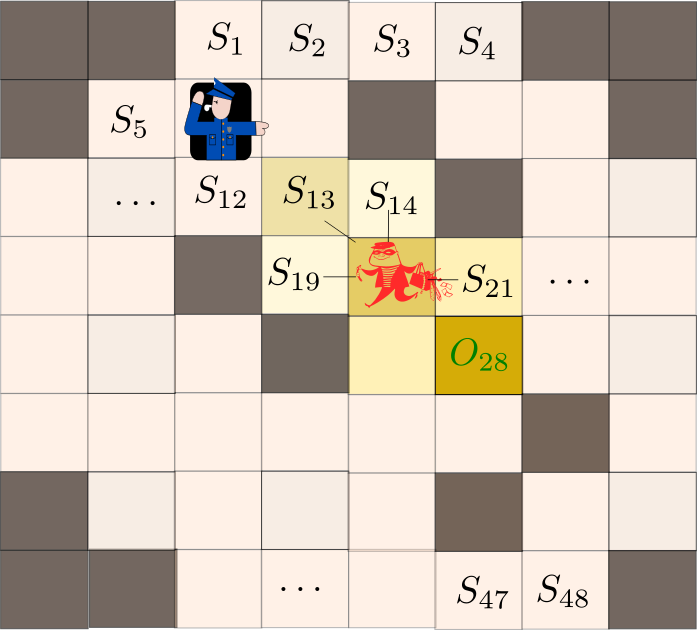
\includegraphics[width=0.9\linewidth]{observation2.png}
			\vspace{-10pt}
			\caption*{\tiny observation 2}
		\end{figure}
	\end{column}
	
	\begin{column}{.34\textwidth}
		\begin{figure}
			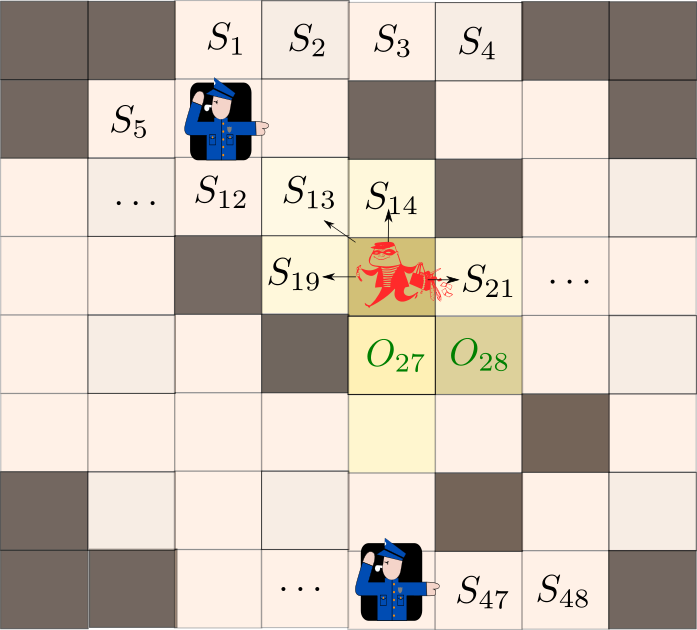
\includegraphics[width=0.9\linewidth]{posterior.png}
			\vspace{-10pt}
			\caption*{\tiny posterior}
		\end{figure}
	\end{column}
\end{columns}	
\end{frame}
\begin{frame}{Network Topology}
	\footnotesize{
		\begin{exampleblock}{}
			Assume that we have $n$ homogeneous agents associated with the nodes of a 
			graph. These agents can communicate with each other under a {\color{blue}time-varying} 
			{\color{blue}undirected} network topology {\color{red}$ G_{k} = \langle \mathcal{V},\mathcal{E}_k\rangle 
				$} where {\color{red}$\mathcal{V}$} and {\color{red}$\mathcal{E}_k$} are the set of graph {\color{red}nodes} and {\color{red}edges} 
			at step $k$ respectively. The node corresponding to the {\color{red}$i^\text{th}$} agent is 
			denoted by {\color{red}$v_i$}. If {\color{red}$(v_i,v_j)\in \mathcal{E}_k$}, it means that agents $i$ and 
			$j$ can communicate directly at step $k$.  The set {\color{red}$\overline{\mathcal{N}}_i$} 
			represent 
			neighbors of node ${v}_i$ that are connected by an edge to $v_i$. The set 
			{\color{red}$\mathcal{N}_i=\overline{\mathcal{N}}_i\cup \{v_i\}$} will also be used in some 
			of the equations. The set {\color{red}$\textsc{CC}_k^i$} represents the set of agents 
			that are {\color{blue}\textit{path-connected}} to agent $i$ at step $k$.
		\end{exampleblock}}
				\begin{figure}
					\centering
					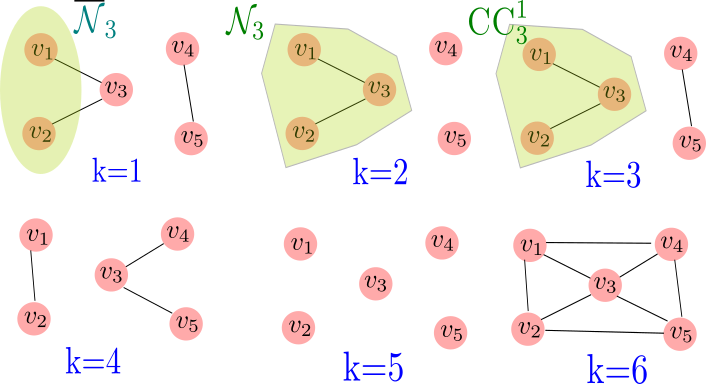
\includegraphics[width=0.50\textwidth]{graph}
				\end{figure}
		
		
\end{frame}
\section{Centralized Estimation on Sensor Networks}
\begin{frame}{Centralized Estimation on Sensor Networks}
	\subsubsection*{Centralized Estimation} In this approach there is a central node in the network that receives observations $\zz{k}{\bIn} \triangleq \{\zz{k}{i}\}^{i\in\bIn}$ from the rest of the nodes. 
	\begin{equation*}
	\label{eq:pred}
	\text{prediction: } \tilde{\pi}_{k} =  \pi_{k-1}\mathcal{P}_{k \vert k-1}.
	\end{equation*}
	\begin{equation*}
	\label{eq:update}
	\text{update: } {\pi}_{k} = \frac{1}{\eta}\tilde{\pi}_{k} \mathcal{O}_k.
	\end{equation*}
	where, $\mathcal{O}_k$ is a $n_s\times n_s$ diagonal matrix of likelihoods $\pr(\zz{k}{\bIn}| \XX[]{k}{})$. 
	
\end{frame}

\section{Distributed Consensus Based Estimation}
\begin{frame}{Distributed Consensus Based Estimation}
	
	If all agents share the same prior information, they can recover the centralized estimator's performance if they can reach a consensus over the product of measurement probabilities.
	{\color{blue}\begin{equation*}
		\tilde{l}_k  = \frac{1}{n} \log \prod_{i=1}^{n} \mathcal{O}_k^i  = \frac{1}{n} \sum_{i=1}^{n} \log \mathcal{O}_k^i = \frac{1}{n} \sum_{i=1}^{n} \tilde{l}_k^i
		\end{equation*}}
	{\color{red}Distributed averaging methods can be applied here.} All the nodes need to reach a consensus over the $\log$ of the joint measurement probabilities (log-of-likelihood).
	Once the consensus is reached, the updated estimate is 
	{\color{blue}
		\begin{equation*}
			{\pi}_{k}  = \frac{1}{\eta}\overbrace{ \underbrace{{\pi}_{k-1}}_{\text{prior}} 
				\mathcal{P}_{k \vert k-1}  
			}^{\text{prediction}}\underbrace{e^{n\tilde{l}_k}}_{\text{likelihood}}.
		\end{equation*}}
\end{frame}

\begin{frame}{Distributed Averaging by Metropolis-Hastings-Markov-Chains}

Consensus over likelihoods using a distributed averaging method based on Metropolis-Hastings Markov Chains (MHMC), {\color{olive}\cite{boyd_fastest_2003}}. 
\begin{align*}
&\vect{\psi}^i(m+1)=\textstyle {\sum\nolimits _{j=1}^{|\mathcal{N}_{i}|}} \gamma_{ij}(m)\vect{\psi}^j(m),\\
& \text{s.t. } \sum_{m}  \gamma_{ij}(m) = 1,\,\,  \vect{\psi}^i(0)=  \tilde{l}_k^i,\nonumber
\end{align*}
to calculate the average of the values on the graph nodes in which $d_{i}(m)=|\overline{\mathcal{N}}^i|$ is the degree of the node $v_i$, and 
\begin{equation*}
\label{eq:mhmc}
\gamma_{ij}(m) =
\begin{cases}
{1\over 1+\max\{d_{i}(m),d_{j}(m)\}}      &  \text{if } (i,j) \in \mathcal{E}_{m}, \\
1-\sum\limits_{{(i,n)} \in \mathcal{E}}\gamma_{in}  &  \text{if } i = j,\\
0 & \text{otherwise}.
\end{cases}
\end{equation*}
With this messaging passing protocol, $$\lim_{m\rightarrow \infty} \vect{\psi}^i(m) = \tilde{l}_k.$$

	
\end{frame}

\begin{frame}{Distributed Averaging by Metropolis-Hastings-Markov-Chains}
	\begin{columns}
		\column{0.50\linewidth}
		How MHMC distributed averaging works in practice
	  \vspace{-11pt}
		\begin{figure}
			\centering
			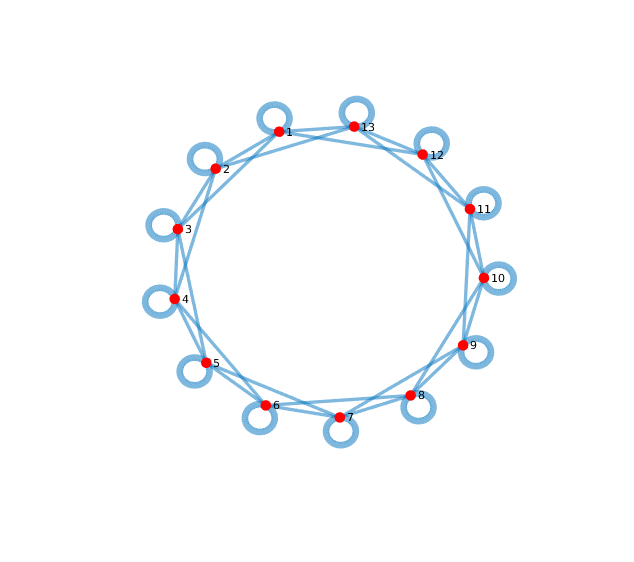
\includegraphics[width=0.50\textwidth, trim={2cm 3cm 2cm 2cm},clip]{graph_for_distributed_averaging}
			\vspace{-11pt}
			\caption*{\tiny Network  Topology}
		\end{figure}
		\vspace{-31pt}
		\begin{figure}
			\centering
			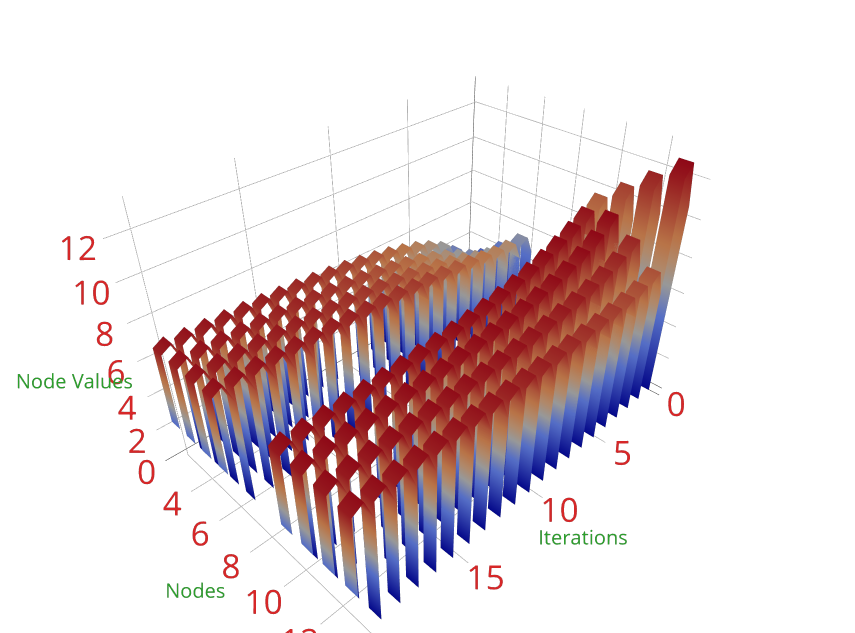
\includegraphics[width=0.70\textwidth, trim={0 0 5cm 2cm},clip]{values_for_dist_av}
			\vspace{-9pt}
			\caption*{\tiny Evolution of node values}
		\end{figure}
		\column{0.50\linewidth}
		{\color{red}Why can't we use distributed averaging when priors are not the same?}
		 
		We have to calculate the following
		\begin{equation*}
		{\pi}_{k}  = \frac{1}{\eta} {\color{orange}\big[\cup_{i=1}^{n}{\pi}^i_{k-1} \big]}
		\mathcal{P}_{k \vert k-1}  
		\color{green}e^{n\tilde{l}_k}.
		\end{equation*}
		We need to avoid double counting of mutual information
		\begin{equation*}
		{\color{orange}{\pi}^i\cup {\pi}^j} = { \color{blue}{\pi}^i + {\pi}^j} - {\color{red}{\pi}^i\cap {\pi}^j}
		\end{equation*}
	\end{columns}
\end{frame}


%	\subsubsection{Conservative approximation of a Probability Mass Function (PMF)} 

\begin{frame}{Conservative Fusion}
	If priors have shared information
	\begin{itemize}
		\item {\color{blue}track the mutual information} (Channel Filter)
		\item {\color{blue}calculate a conservative approximation of fused priors}
	\end{itemize}
	\begin{exampleblock}{Conservative Approximation of a PMF}
	A set of sufficient conditions that a PMF $\tilde{\pr}(\vect{X})$ has to satisfy in order to be a conservative approximation of another PMF $\pr(\vect{X})$, which are ({\color{olive}\cite{bailey2012conservative}})
	\begin{itemize}
		\item {\color{red}The non-decreasing entropy property},
		$$\begin{aligned}
		\text{H}(\pr(\vect{X})) \leq \text{H}(\tilde{\pr}(\vect{X}))
		\end{aligned}$$
		\item {\color{red}The order preservation property that}, $\forall \vect{x}_i,\vect{x}_j\in\vect{X}$,
		$$\begin{aligned}
		\pr(\vect{x}_i) \leq \pr(\vect{x}_j) \ \text{iff}\  \tilde{\pr}(\vect{x}_i) \leq \tilde{\pr}(\vect{x}_j) 
		\end{aligned}$$
	\end{itemize}
	\end{exampleblock}
\end{frame}


\begin{frame}{Conservative Fusion}
		\begin{exampleblock}{Conservative Fusion of two PMFs}
				Two probability distribution functions $\pr_a(\vect{X | \vect{I}_a})$ and $\pr_b(\vect{X} | \vect{I}_b)$ can be fused together following the {\color{blue}\emph{Geometric Mean Density Rule (GMD)}}
				\begin{equation*}
				\begin{aligned}
				\pr_c(\vect{X})&= \frac{1}{\eta_c} \pr_a(\vect{X| \vect{I}_a})^\omega \pr_b(\vect{X| \vect{I}_b})^{1-\omega}\\
				=& \frac{1}{\eta_c} \pr_a(\vect{X| \vect{I}_a} \setminus \vect{I}_b)^\omega \pr_b(\vect{X| \vect{I}_b} \setminus \vect{I}_b)^{1-\omega} {\color{green}\pr_a(\vect{X| \vect{I}_a} \cap \vect{I}_b)},\\
				\end{aligned}
				\end{equation*}
		\end{exampleblock}
	
	\begin{exampleblock}{}
		Several criteria have been proposed to choose the $\omega_i$. One such criteria is \citep{ajgl2015design}
		\begin{equation*}
		\label{eq:crit}
		\tilde{\pi}=\arg\min_{\pi}\max_i\{\mathcal{D}(\pi\Vert \tilde{\pi}^{i})\}, \end{equation*}
		in which the $\mathcal{D}(\pi\Vert \tilde{\pi}^{i})$ is the {\color{red}Kullback-Leibler divergence} between densities $\pi$ and $\tilde{\pi}^i$.
	\end{exampleblock}
\end{frame}
\section{Iterative Conservative Fusion}
\begin{frame}{Iterative Conservative Fusion}
At first iteration of consensus, {\color{blue}$m=0$}, for {\color{blue}each agent $j$}, take the most recent local estimate {\color{blue}${\pi}_{k-1}^j$} and calculate the prediction {\color{blue}$\tilde{\pi}_k^j$}. 
Initialize the local 
consensus variable using local prediction and local observation {\color{blue}$\mathcal{O}_k^j$}
{\color{brown} $$\mathcal{\phi}^j(0) 
=\frac{1}{\eta_i}\tilde{\pi}_k^j\mathcal{O}_k^j. $$ }
Iteratively update 

\begin{equation*}
{\color{brown}\mathcal{\phi}^i(m + 1) = 	\frac{1}{\eta^*} {\prod\nolimits_{j \in {\cal N}^{i}(m)} }  \big[\mathcal{\phi}^j(m)\big]^{\omega_{j}^*}.}
\end{equation*}
After convergence ( {\color{blue}
$\textsc{CC}^i_k$} is the set of agents that form a 
{\color{blue}connected 
group} with agent $i$ at step $k$)
\begin{equation*}
{\color{brown}
\lim\limits_{m\rightarrow 
	\infty}\vect{\phi}^{i}(m) = \mathcal{\phi}^*=	
\frac{1}{\eta} 
{\prod\nolimits_{j \in \bIs{\suf{CC}^i_k} } }  
\big[\mathcal{\phi}^j(0)\big]^{\omega_{j}^*},\forall i \in \textsc{CC}^i_k.}
\end{equation*}

\end{frame}

\begin{frame}{Why Hybrid Algorithm?}
\centering
%\vspace{-100pt}
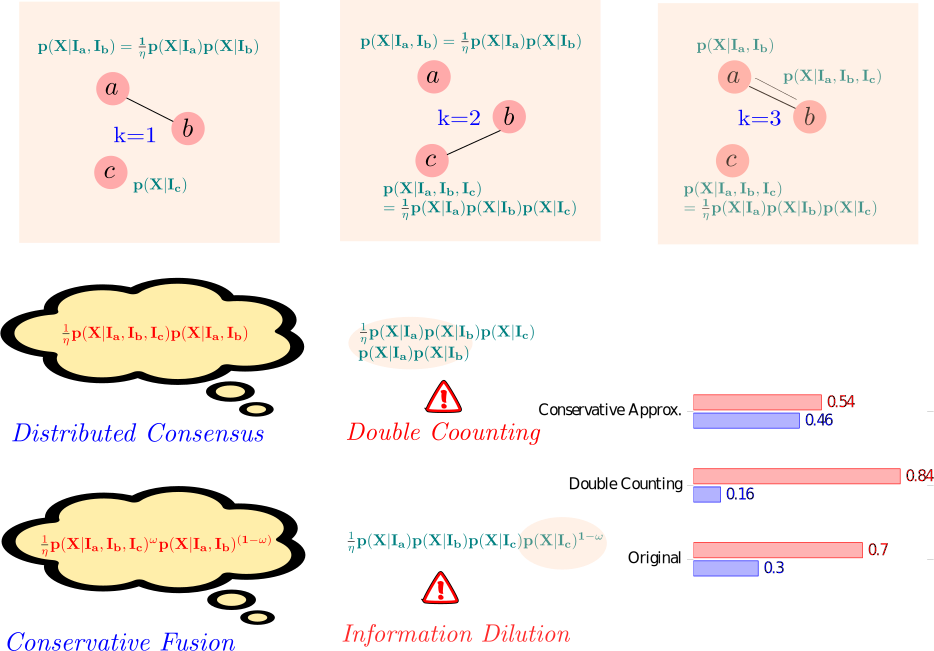
\includegraphics[width=.9\columnwidth]{scenario3}
\end{frame}
\begin{frame}{Hybrid Algorithm}
	
{\color{red} Recap)}
We wanted to get as close as possible to centralized estimator
	{\color{blue}
		\begin{equation*}
		{\pi}_{k}  = \frac{1}{\eta} {{\pi}_{k-1}}
			\mathcal{P}_{k \vert k-1}  
		\prod_{i=1}^{n} \mathcal{O}_k^i
		= \frac{1}{\eta}\overbrace{ \underbrace{{\pi}_{k-1}}_{\text{prior}} 
			\mathcal{P}_{k \vert k-1}  
		}^{\text{prediction}}\underbrace{{\color{green}e^{n\tilde{l}_k}}}_{\text{likelihood}}.
		\end{equation*}}
{\color{red} If} the network remained connected all the time and {\color{red} If} enough time was given for consensus algorithm to converge, agent priors matched the prior of the centralized estimator  and distributed averaging {\color{red}alone} could solve the DSE problem.
{\color{red} Iterative Conservative Fusion} would help with unequal prior, network disconnection and, avoiding double counting.
\begin{equation*}
 	{\pi}_{k}^*=	
	\frac{1}{\eta} 
	{\color{blue}{\prod\nolimits_{j \in \bIs{\suf{CC}^i_k} } }  
	\big[{\pi}^i_{k-1}\big]^{\omega_{j}^*}}
		\mathcal{P}_{k \vert k-1}
		{\color{blue}{\prod\nolimits_{j \in \bIs{\suf{CC}^i_k} } }\big[\mathcal{O}_k^i\big]^{\omega_{j}^*}		
		}.
\end{equation*}
Hybrid of {\color{blue}ICF on priors} and {\color{orange} Distributed Averaging on Likelihoods} will give us
\begin{equation*}
{\pi}_{k}^*=	
\frac{1}{\eta} 
{\color{blue}{\prod\nolimits_{j \in \bIs{\suf{CC}^i_k} } }  
	\big[{\pi}^i_{k-1}\big]^{\omega_{j}^*}}
	\mathcal{P}_{k \vert k-1}
	{\color{orange}{\prod\nolimits_{j \in \bIs{\suf{CC}^i_k} } }\big[\mathcal{O}_k^i\big]}		.
\end{equation*}
\end{frame}

\section{Hybrid Algorithm}
\begin{frame}{Hybrid Algorithm}
	\scalebox{.6}{                        %new code
		\begin{algorithm}[H]
			\label{alg:inf-predict}
			\SetKwInOut{Input}{Input}
			\SetKwInOut{Output}{Output}
			\Input{${\pi}^i_{k-1}$ }
			\caption{Hybrid Method}
			Use \eqref{eq:update} to calculate  $\tilde{\pi}^i_{k}$
			%$[{y}_j^-(t_0) ,{Y}_j^-(t_0)] =\texttt{PRED}[{y}_j(t_0),{Y}_j(t_0)]$ 
			
			Collect local observation ${z}^i_{k}$ and calculate ${\mathcal{O}}^i_{k}$ 
			and $\tilde{l}_k^i$
			
			Initialize consensus variables
			\begin{equation*}
			\YY[]{0}{i} = \tilde{\pi}^i_{k}, \quad \yy[]{0}{i} = \tilde{l}_k^i
			\end{equation*}
			
			$m=0$\\
			\While{\texttt{NOT CONVERGED}} 
			{ $\texttt{BROADCAST}[ \yy[]{m}{i}, \YY[]{m}{i}]$\\
				$\texttt{RECEIVE}[ \yy[]{m}{j}, \YY[]{m}{j} ] \quad \forall j \in 
				\mathcal{N}^i$\\	
				Collect received data 
				\begin{equation*}
				\mathcal{C}^i(m)=\{  \YY[]{m}{j \in  \mathcal{N}^i} \}, \quad 	
				\mathcal{M}^i(m)=\{  \yy[]{m}{j \in  \mathcal{N}^i} \}
				\end{equation*}
				
				Do one iteration of ICF on consensus variables for local prior 
				information $\mathcal{C}^i_m$
				$$ \YY[]{m+1}{i}=\texttt{ICF}(\mathcal{C}^i(m))$$\\
				Do one iteration of MHMC on consensus variables for new 
				information 		$$ \yy[]{m+1}{i}=\texttt{MHMC}(\mathcal{M}^i(m))$$\\
				$m=m+1$\\
			}
			Calculate the posteriors according to:
			\begin{equation*}
			{\pi}^i_{k} = e^{|\textsc{CC}^j_k|\yy[]{m}{i}}\YY[]{m}{i}
			\end{equation*}
		\end{algorithm}
	}
\end{frame}

%\begin{frame}{Experimental Results}
%\rc{The effect of disconnection on estimation performance}
%
%\begin{columns}
%\begin{column}{.50\textwidth}
%		\begin{figure}[t]
%		\centering
%		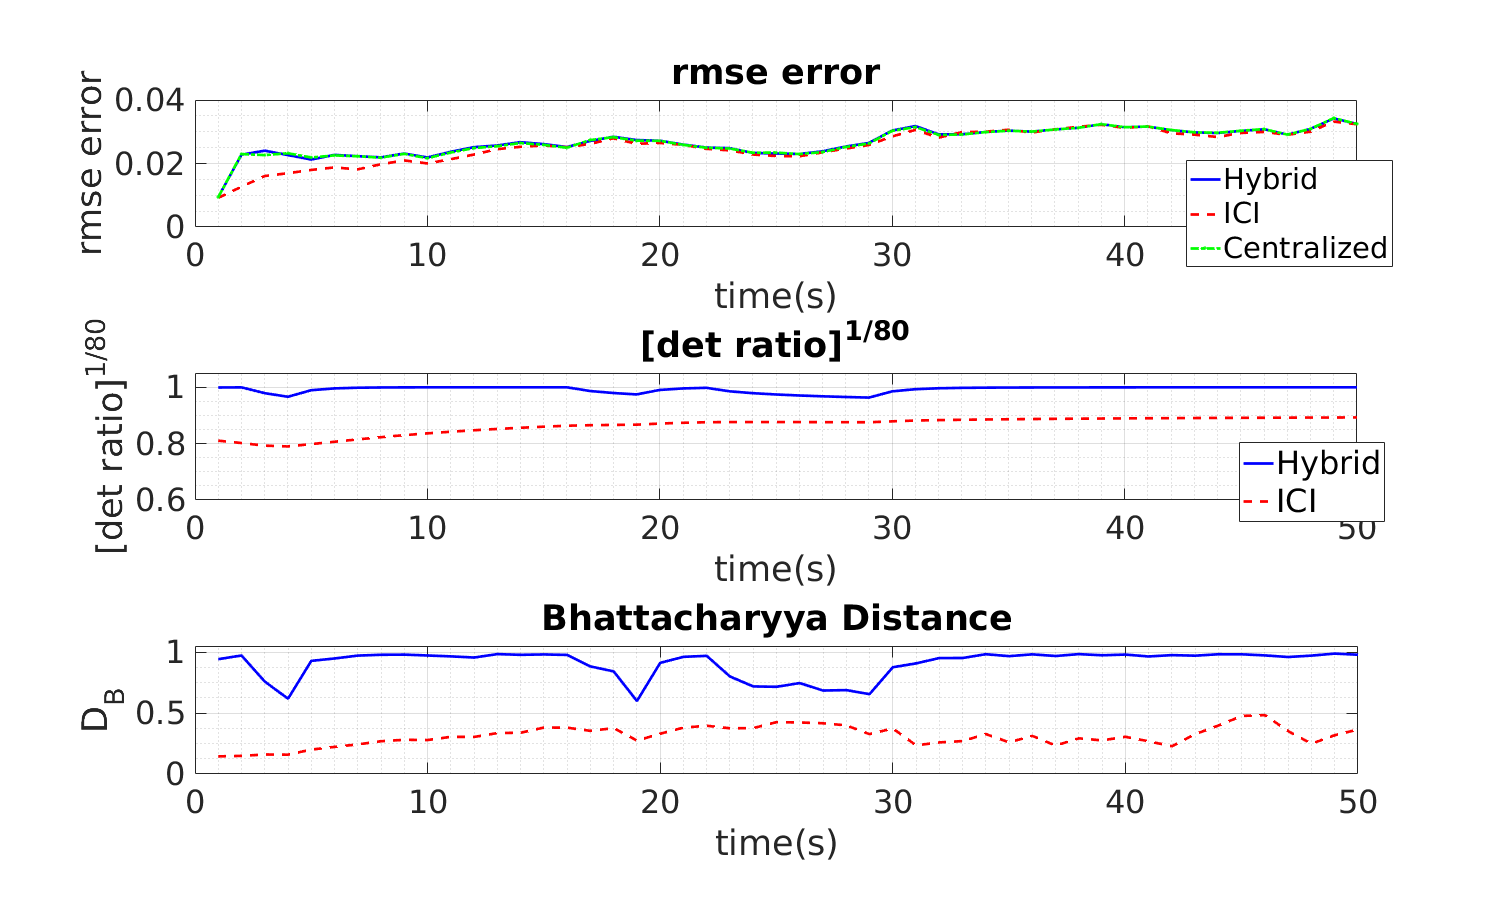
\includegraphics[width=1\linewidth]{long_run_paper3.png}
%%		{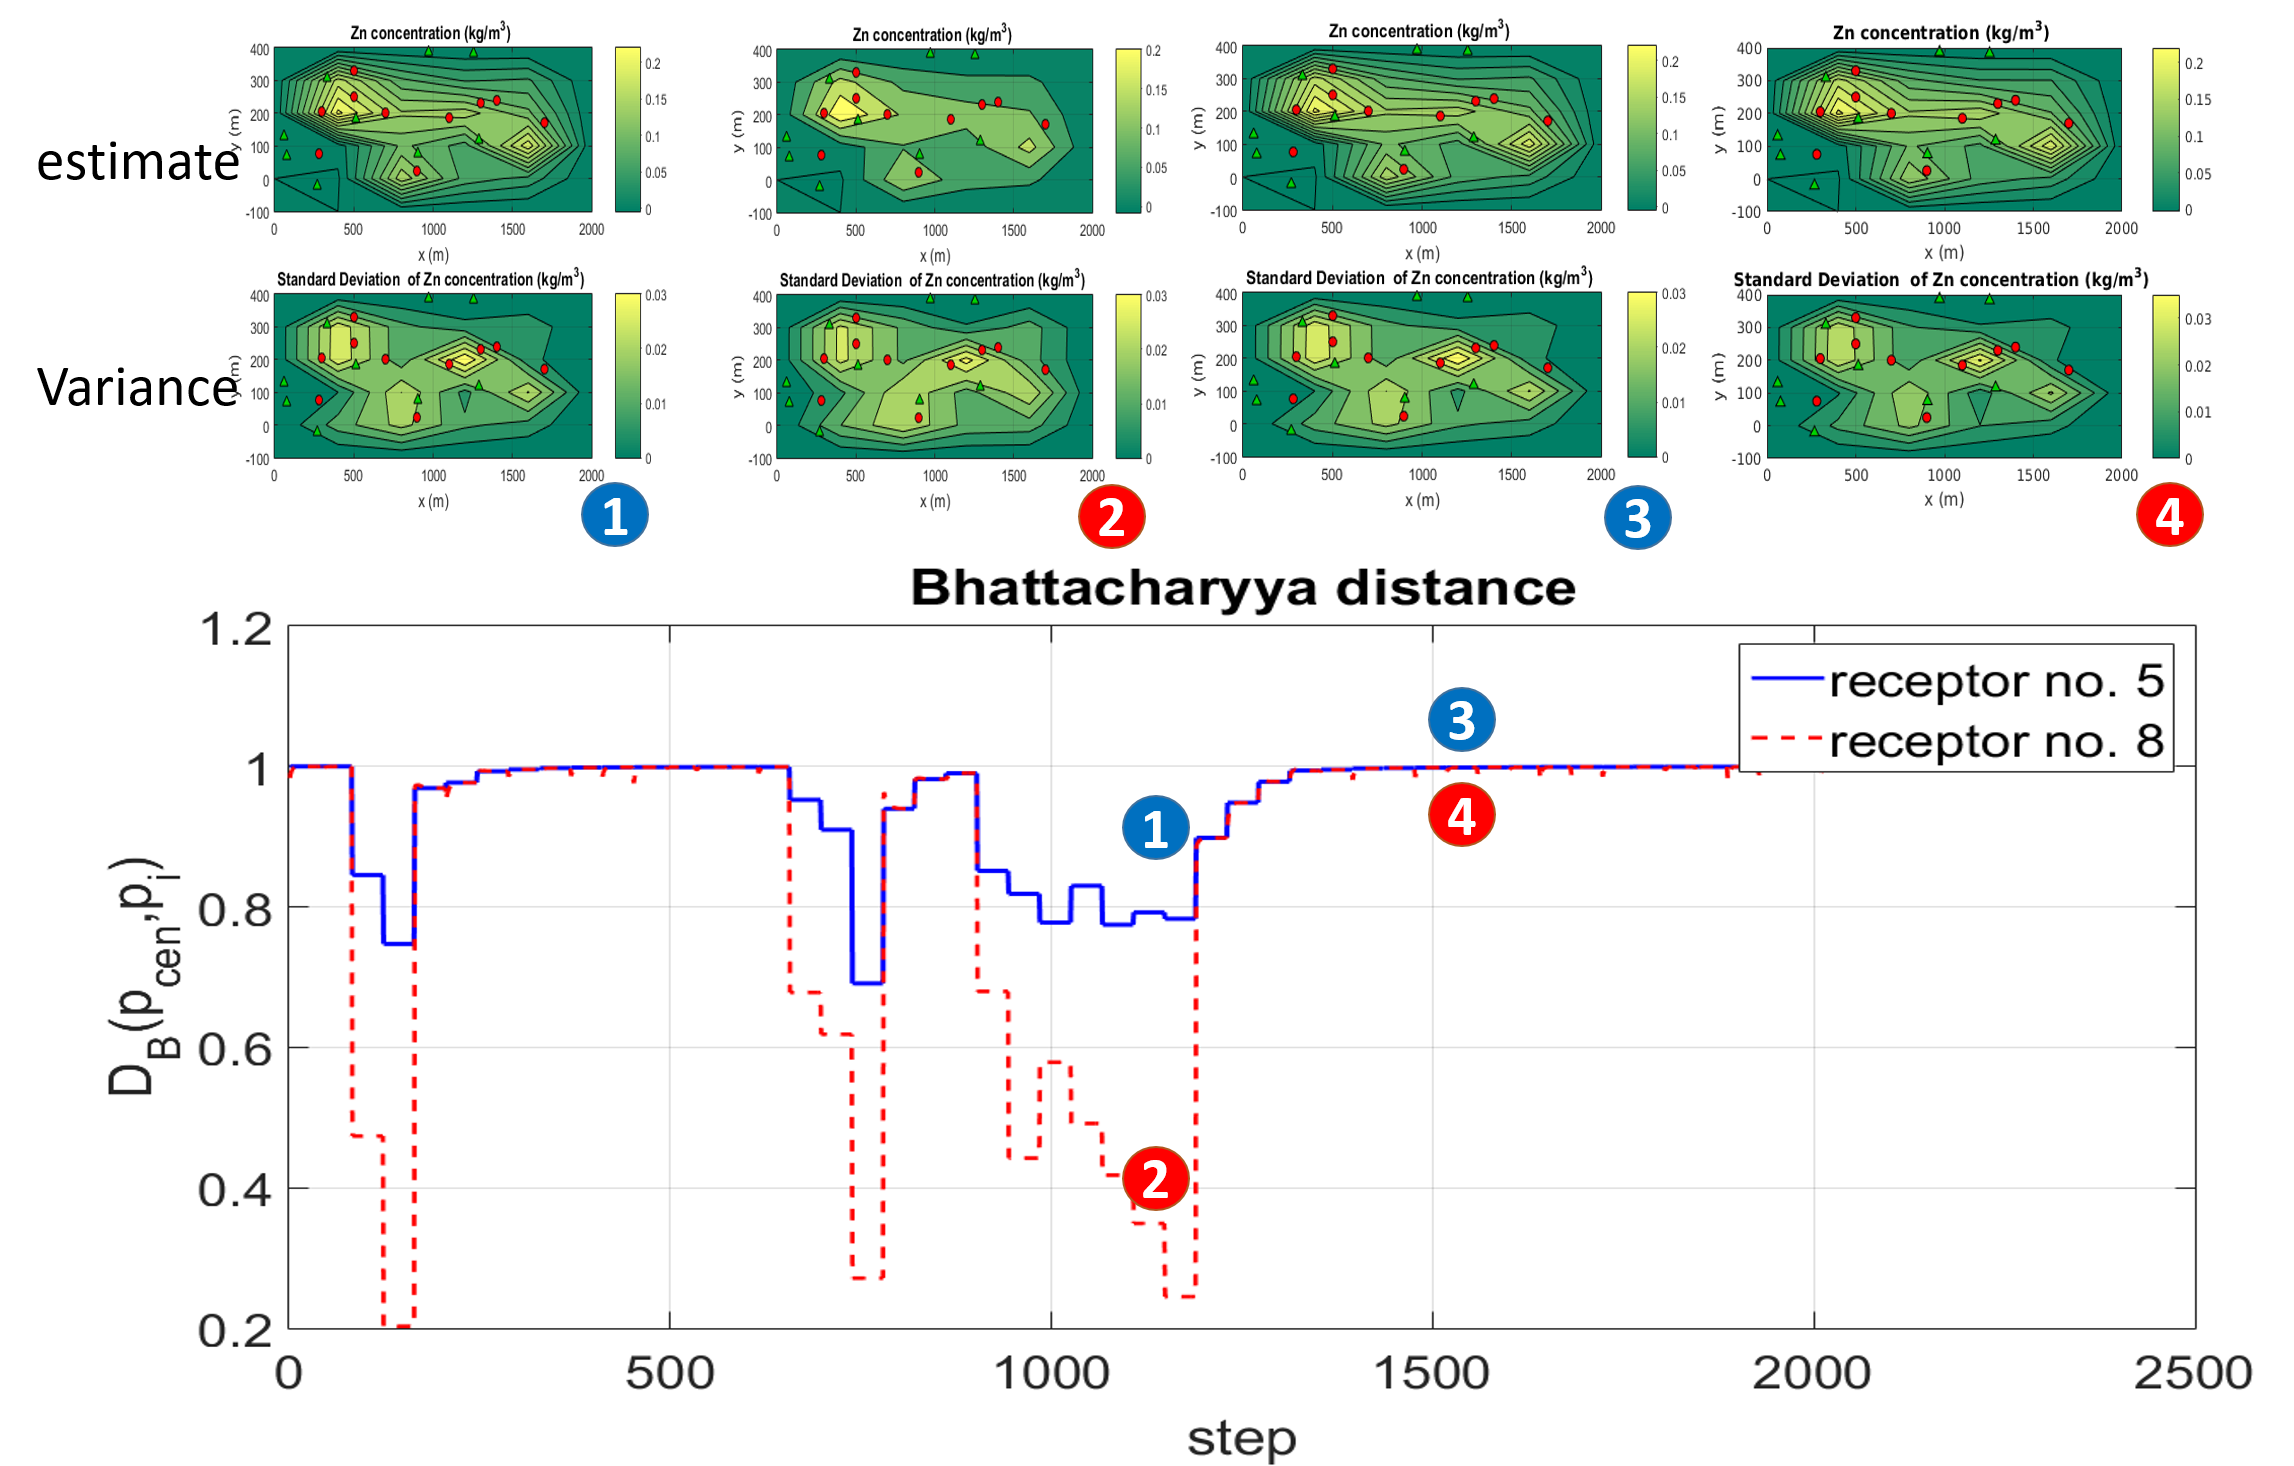
\includegraphics[width=1.2\linewidth]{long_run_comp.png}} 
%		\label{fig:sim_error_comp}
%		\end{figure}	
%\end{column}
%\begin{column}{.50\textwidth}
%\begin{figure}[T]
%\centering
%{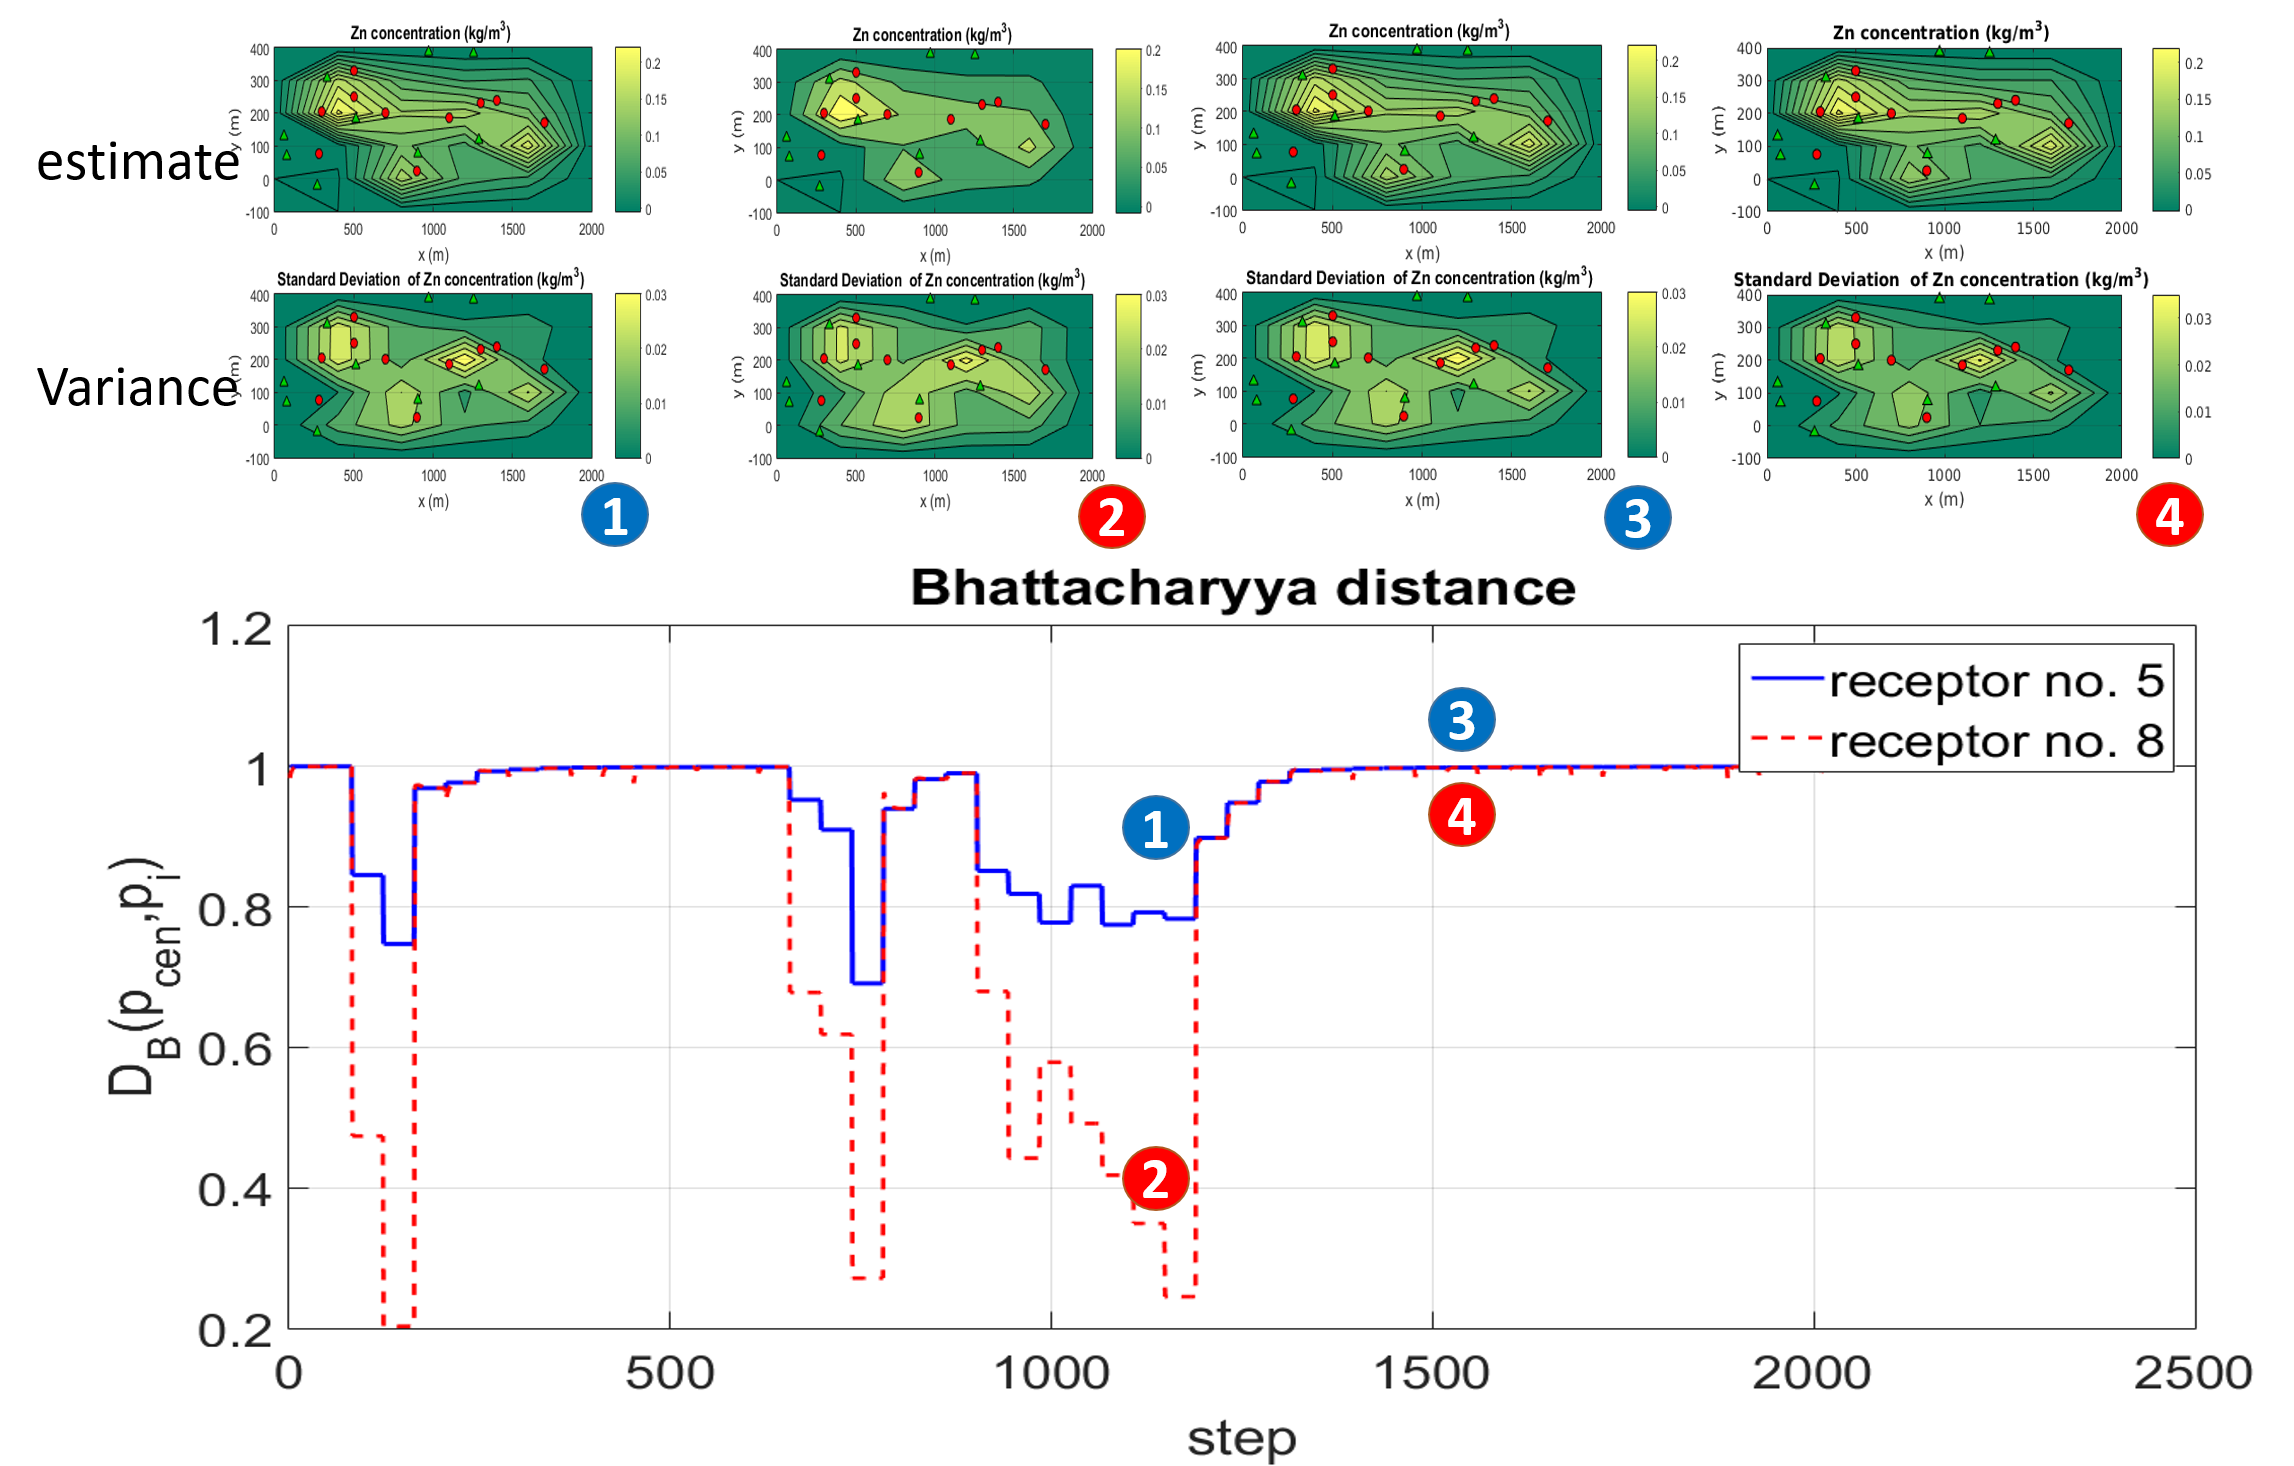
\includegraphics[width=1\linewidth]{long_run_comp.png}} 
%\begin{center}
%\end{center}
%\label{fig:motivating_example_vert}
%\end{figure}
%\end{column}
%\end{columns}
%\begin{figure}[T]
%\vspace{-15pt}
%\centering
%{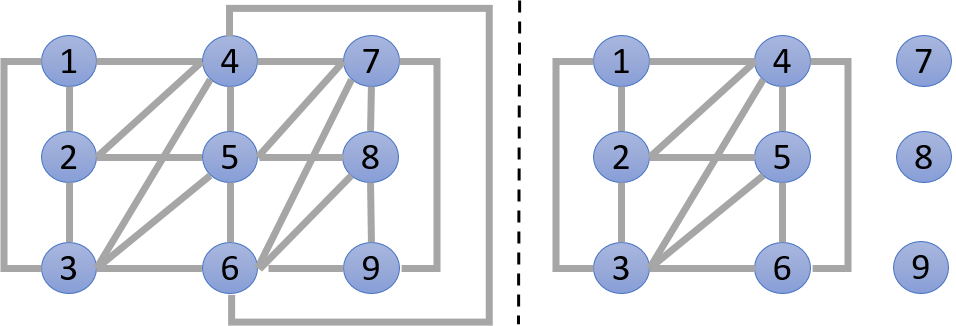
\includegraphics[width=0.5\linewidth]{top_ppt.png}} 
%	\caption{\footnotesize Topology of the Network when all receptors are connected (left) and when receptors 7,8 and 9 get disconnected from the rest of the group (right). }
%\begin{center}
%\end{center}
%\label{fig:motivating_example_vert}
%\end{figure}
%\end{frame}

%\begin{frame}[plain,c]
%	%\frametitle{A first slide}
%	\begin{center}
%		\Huge Finite State System + non-Gaussian Noise 
%	\end{center}
%\end{frame}

\section{Experimental Results}
\begin{frame}{Experiments: Multi Agent Tracking}
	\begin{columns}
		\column{0.50\linewidth}
		\vspace{-11pt}
		\begin{figure}
			\centering
			{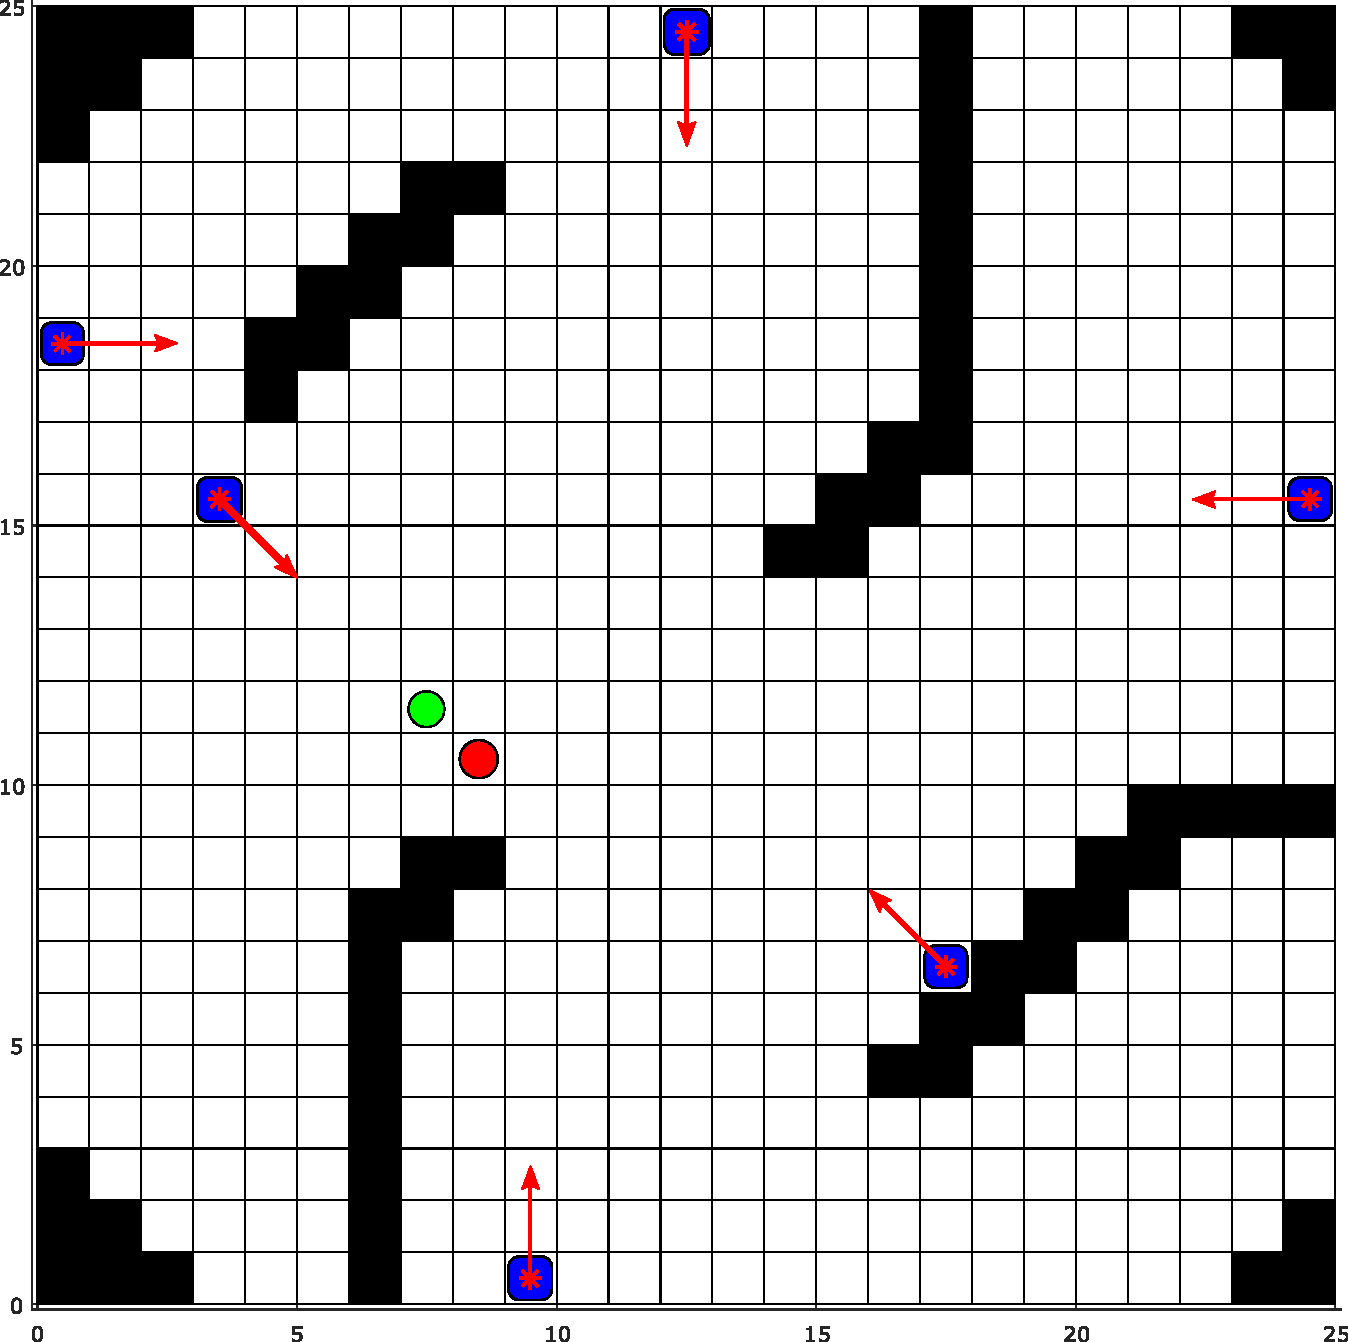
\includegraphics[width=.69\columnwidth]{exp1_Corrected2.pdf}}
%		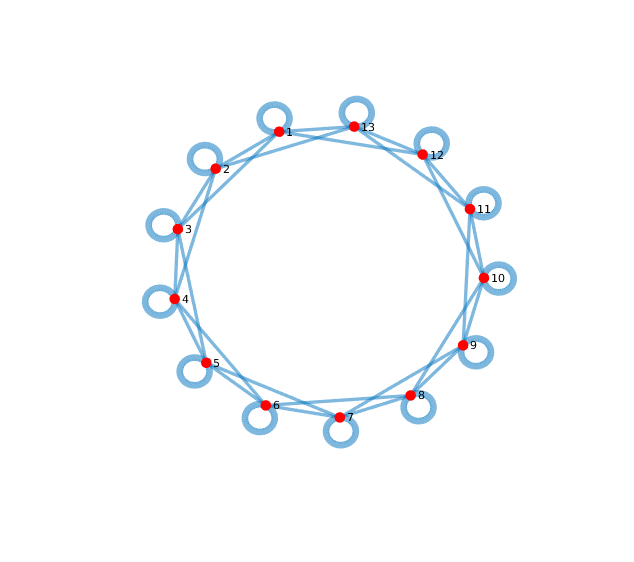
\includegraphics[width=0.50\textwidth, trim={2cm 3cm 2cm 2cm},clip]{graph_for_distributed_averaging}
				\vspace{-5pt}
			\caption*{\tiny Multi Agent Tracking Scenario}
		\end{figure}
				\vspace{-20pt}
						\tiny{
				\begin{exampleblock}

			To quantify differences, we use the 
			{\color{red}Bhattacharyya coefficient (BC)} {\color{olive}\cite{bhattacharyya1946measure}} between the estimation results and 
			the 
			centralized estimator. BC can be used to evaluate 
			the 
			{\color{orange}similarity of two probability mass functions}, $\pi_1(\vect{X}), 
			\pi_2(\vect{X})$ as:
			{\color{blue}
				\begin{equation*}
				\textstyle BC(\pi_1(\vect{X}),\pi_2(\vect{X})) = \sum_{\vect{x}\in 
					\vect{X}}\sqrt{\pi_1(\vect{x}) \pi_2(\vect{x})}.
				\end{equation*}}
			In the case of complete similarity, $p_1= p_2$, we have $BC(p_1,p_2)=1$. Moreover, 
			$BC(p_1,p_2)=0$ describes maximal dissimilarity.
		\end{exampleblock}}
		\column{0.50\linewidth}
		\begin{figure}
			\centering
			{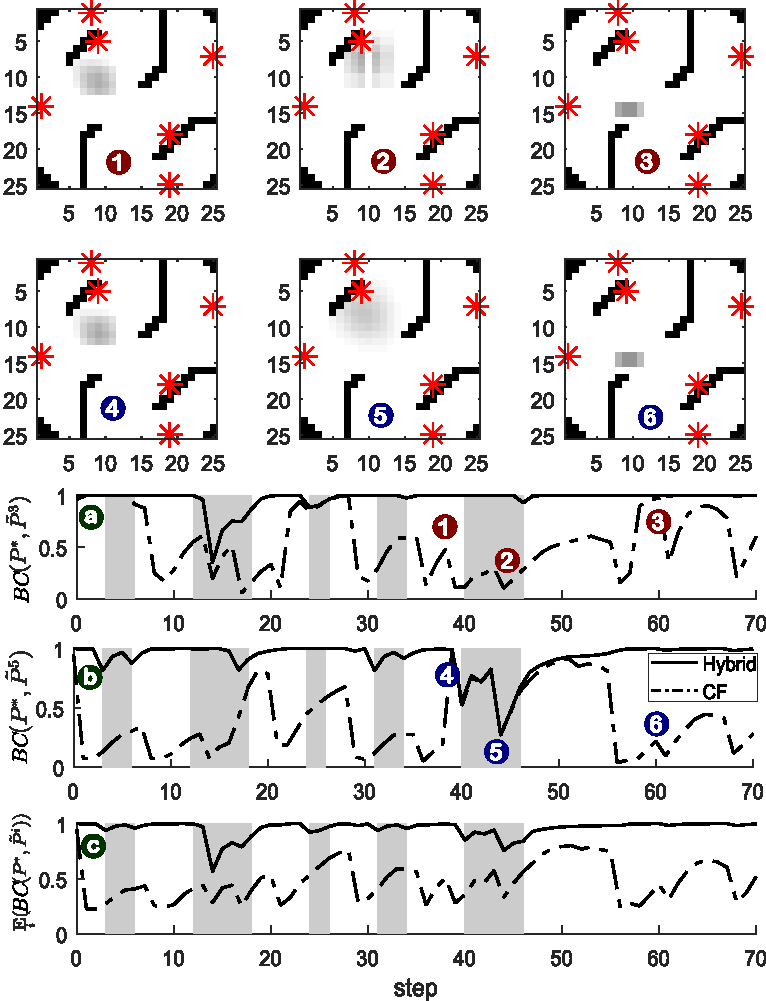
\includegraphics[width=0.85\textwidth, trim={0cm 0cm 0cm 0cm},clip]{./figs/exp2.pdf}}
			\caption*{\tiny Estimation performance in the tracking example}
		\end{figure}
	\end{columns}
\end{frame}
\begin{frame}{Experiments: Random High Dimensional HMM}
				\begin{figure}
					\centering
					{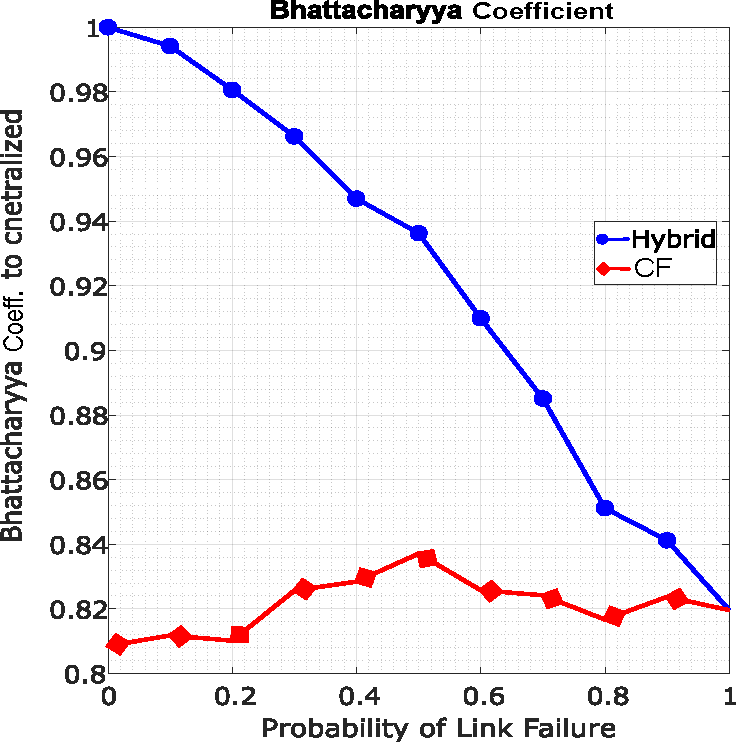
\includegraphics[width=0.4\columnwidth]{perf_measures_NGMD_GMD_curve7_corrected.pdf}}
				\end{figure}
				
			\footnotesize{
				\begin{exampleblock}
					
					In a second experiment we have evaluated the robustness of the proposed method 
					for networks with different likelihoods of link failure. We report the 
					Bhattacharyya coefficient vs. link failure 
					probability 
					for a general decentralized HMM with a network of size 20 and state size 30 
					with each node roughly connected to 10\% of the other nodes. We simulate the 
					system multiple times, each time for 150 time steps but with different 
					probability of link failure. At each step, given a probability of failure for each link, 
					some links in the graph will randomly be disconnected.
				\end{exampleblock}}
	
\end{frame}

\begin{frame}[plain,c]
	%\frametitle{A first slide}
	\begin{center}
		\Huge Questions ?
	\end{center}
\end{frame}
\begin{frame}[allowframebreaks]
	\frametitle{References}
%	\bibliographystyle{plainnat}
	\bibliographystyle{apalike} 
	
%	\bibliographystyle{IEEEtran}
	\bibliography{RSS_2017_2}
\end{frame}


% All of the following is optional and typically not needed. 

\end{document}


